
\documentclass[a4paper,10pt,twoside]{cpc-hepnp}

\usepackage{multicol}

\usepackage{graphicx}
\usepackage{booktabs}
\usepackage{amssymb,bm,mathrsfs,bbm,amscd}
\usepackage[tbtags]{amsmath}
\usepackage{lastpage}
\usepackage{CJK}

\usepackage{booktabs}  %  ???????
\usepackage{amsfonts}
\usepackage{subfigure}

\begin{document}
%\begin{CJK*}{GBK}{song}
\begin{CJK*}{GB}{gbsn}

\fancyhead[c]{\small PREPARED FOR SUBISSION TO CPC} \fancyfoot[C]{\small 010201-\thepage}

\footnotetext[0]{}




%\title{JUNO Calibration Strategy }
\title{Design of JUNO Calibration system}

\author{%
      %Author1$^{1,2;1)}$\email{someone@sjtu.edu.cn}%
\quad someone$^{1)}$\email{someone@sjtu.edu.cn}%
%\quad LI Da-Ming(�����)$^{1}$
%\quad F. Jone$^{2}$
}
\maketitle


\address{%
$^1$ School of Physics and Astronomy, Shanghai Jiao Tong University, Shanghai Key Laboratory for Particle Physics and Cosmology, Shanghai, 200240, China  \\
%$^2$ {\bf Example}: Institute of High Energy Physics, Chinese Academy of Sciences, Beijing 100049, China\\
}


\begin{abstract}
Jiangmen Underground Neutrino Observatory (JUNO) is a spherical-tank (35.4 m diameter) neutrino detector filled with 20 kton liquid scintillator. It is located 700 m underground in Jiangmen City, Guangdong province, China. The primary purpose of JUNO is to measure the neutrino mass hierarchy (MH). So a high physics requirement is purposed for both energy scale and resolution. The overall energy resolution should be better than 3\% and uncertainty of the energy scale should be less than 1\%. In order to achieve this physics requirement, a design of calibration system is purposed. The design includes types of source, geometries of source design, simulation and expected results.
\end{abstract}


\begin{keyword}
JUNO,Calibration,Simulation,Radioactive source
\end{keyword}

%\begin{pacs}
%1--3 PACS(Physics and Astronomy Classification Scheme, http://www.aip.org/pacs/pacs.html/)
%\end{pacs}


%\footnotetext[0]{\hspace*{-3mm}\raisebox{0.3ex}{$\scriptstyle\copyright$}2013
%Chinese Physical Society and the Institute of High Energy Physics
%of the Chinese Academy of Sciences and the Institute
%of Modern Physics of the Chinese Academy of Sciences and IOP Publishing Ltd}%


\begin{multicols}{2}



\section{Introduction}
\subsection{Motivation of calibration}
JUNO is a muti-purpose neutrino detector, and the main purpose of JUNO is to determine the neutrino mass hierarchy. As a medium baseline reactor anti-neutrino detector, 53 km from the Yangjiang and Taishan NPP, it can resolve the MH in the neutrino oscillation. But this requires very high precise measurement on both energy resolution and scale. Based on Ref.~\cite{lab1}, the energy resolution of JUNO detector should be better than 3\% and the uncertainty of energy scale should be better than 1\%.

%\begin{center}
%	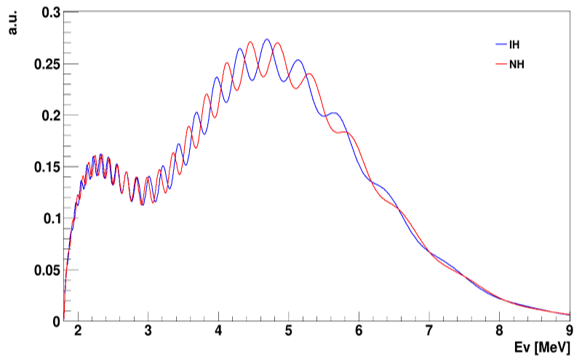
\includegraphics[width=3.0in]{IBD.png}
%	\figcaption{\label{IBD_spe}The IBD spectrum}
%\end{center}

However, due to the LS transmittance and total reflection at CD boundary, connection bar and so on, the response of detector is not uniform, and the non-uniformity effect will worsen the detector energy resolution, so we need to correct the non-uniformity with calibration system to make the energy resolution good enough to meet the physics requirement. 
Fig.~\ref{mono_energy} shows the simulation of 1 MeV e+ uniformly in CD without correction, the energy  resolution is ~7\%, which doesn't meet the physics requirement of JUNO. So A calibration strategy for non-uniformity correction is very necessary.


The other effect is about energy non-linearity of detector response. The quenching of LS is different for different energy, and even with the same energy, e-, e+ and gamma still have different quenching, so the quenching of LS is energy and particle dependent. Reference to Ref.~\cite{lab1}, the incorrect energy scale will give wrong MH sensitivity (increase or decrease), so we need various sources to calibrate it.

\subsection{Calibration system}

\begin{center}
	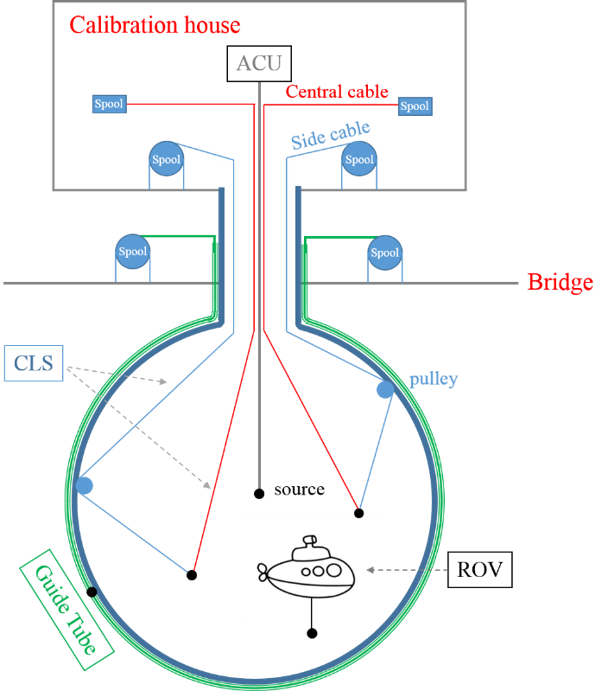
\includegraphics[width=3.0in]{calibration_system.png}
	\figcaption{The overview of calibration system}
	\label{overview_calibration_system}
\end{center}
The deployments systems of calibration sources include ACU, CLS, GT, ROV as shown in Fig~\ref{overview_calibration_system}. For ROV and CLS, we will use independent positioning system to determine the position of calibration source.

The ACU is developed to do calibration along the central axis of CD, which is very similar to the ACU used in Daya Bay experiment. There are 4 spools installed on the turntable. Three routine sources and one exchangeable source are installed on the ACU. The three routine sources include one gamma source (K40), one neutron source (Am-C) and one laser source. The calibration with ACU can coverage central axis of CD, with high precision of position control. The energy scale of CD can be used with neutron source deployed by ACU to the CD center.    
\subsubsection{Cable loop system (CLS)}
The CLS is necessary since we need to have a better understand of detector non-uniformity.
The CLS mainly consist of two cables, side cable and central cable. Controlling the lengths of two cable, we can deploy the sources to scan one vertical plane area.
Two sets of CLS with different anchor positions are purposed to increase the scanning area. 
   
\subsubsection{Guide Tube (GT)}
Since the source cannot reach some boundary area of CD duo to mechanical limit, a Guide Tube calibration system was purposed. The guide tube will be out of CD. With the GT, we can position the calibration source along the surface of CD to obtain a better understand of boundary effect. 
\subsubsection{Remotely Operated Under-liquid-scintillator Vehicles (ROV)}
ROV is 3D scanning system, meaning that we can move the calibration to nearly everywhere in the CD. ROV is not a routine calibration system, but it still essential as a supplement of ACU, CLS, and GT.
\subsubsection{Positioning system}
During the non-uniformity correction, we should precisely know the position of calibration points, so it's very important to get the position of calibration source.

However, it's difficult to determine position of source based on length of cable. Due to self-weight, the cable is not straight, we cannot calculate the position of source with naive trigonometric relation. So it's necessary to use independent position system to determine the source position.  The requirement of precision of source position is ~3 cm compared with that the requirement of vertex reconstruction is ~ 10 cm.

\section{Introduce of simulation}
\subsection{Offline sniper}

\subsection{Introduction of source geometry}
There are three parts for every radioactive source,including source enclosure, weight and quick connector, as shown in Fig.~\ref{source_weight_QC}. The total distance from top to bottom is 50 cm, and two cables are used to combine them together. The length of every cable is about 20 cm, which can make sure small shadowing effect from weight and quick connector. 


Fig.~\ref{gamma_source} is the geometry of gamma source. The internal part is stainless steel to seal the source. Both diameter and height of the SS are 6mm, which is very small to decrease the energy loss, with two loops at top and bottom to attach the cable. The outer is the PTFE shell to increase the reflectivity to minimize the photon loss. 

\begin{center}
	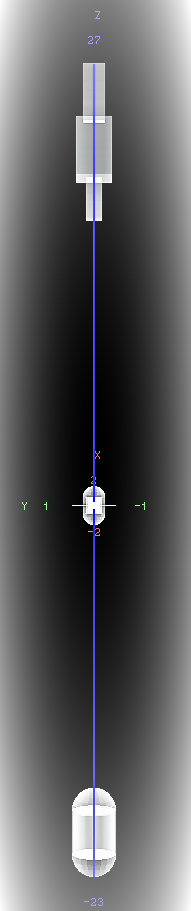
\includegraphics[width=0.8in]{source_geometry1.png}
	\figcaption{Overview of source, weight and quick connector}
	\label{source_weight_QC}
\end{center}

\begin{center}
	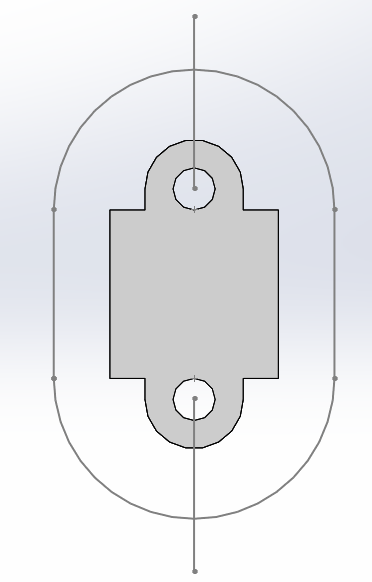
\includegraphics[width=1.5in]{source_geometry2.png}
	\figcaption{Geometry of gamma source}
	\label{gamma_source}
\end{center}


The neutron enclosure is different from gamma since smaller neutron source is not safe and necessary, as shown in Fig.~\ref{neutron_source}. Both diameter and height of neutron source are 8 mm. The source is in a stainless steel (SS) tube. There are two SS pins respectively in top and bottom of the tube. The outer is the PTFE shell just same as gamma source. Fig.~\ref{neutron_prototype} shows the prototype of neutron source which has been tested in Daya Bay Detector. 

\begin{center}
	%\centering
	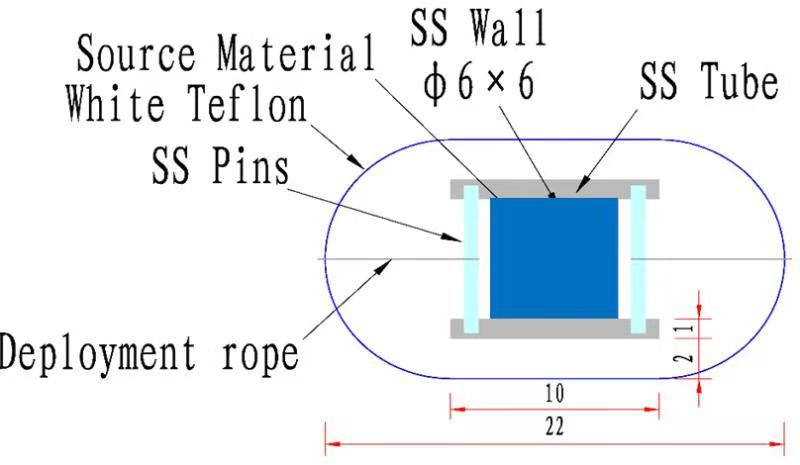
\includegraphics[width=3in]{source_geometry3.png}
	\figcaption{Geometry of neutron source}
	\label{neutron_source}
\end{center}

\begin{center}
	%\centering
	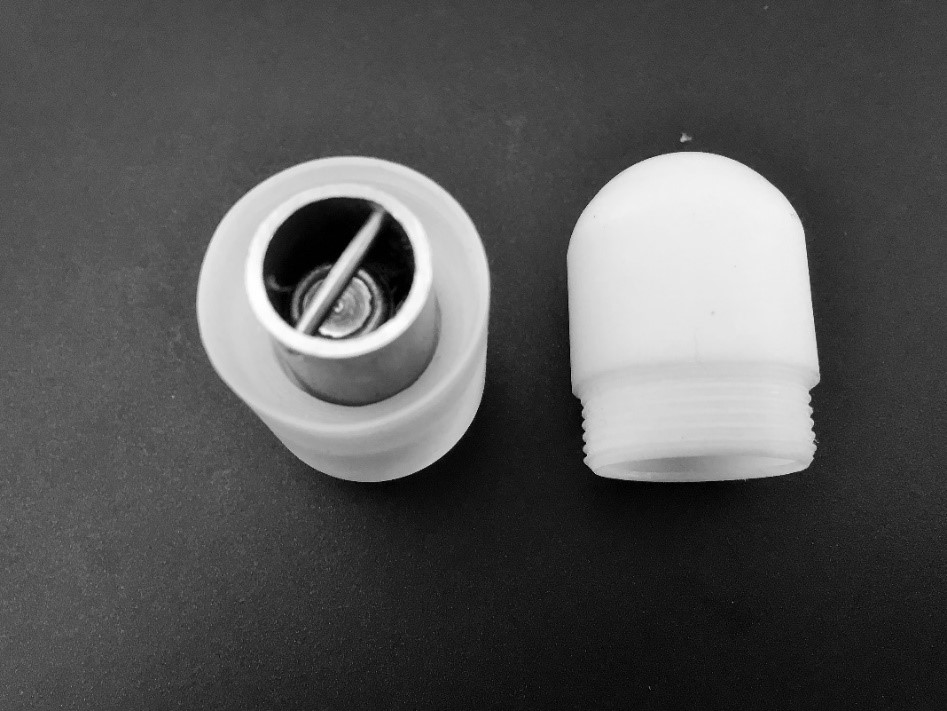
\includegraphics[width=3in]{neutron_source_prototype.jpg}
	\figcaption{Prototype of neutron source}
	\label{neutron_prototype}
\end{center}

\subsection{Calibration source}
The radioactive sources include routine gamma and neutron sources. The detail of calibration sources and correlated energy is shown in table~\ref{radioactive_source}

\begin{center}
	\tabcaption{Radioactive sources}
	\footnotesize
	\begin{tabular}{c@{\extracolsep{\fill}}ccccc}
		\toprule  % ???
		Source & Type & Radiation\\ 
		\midrule  % ???
		$^{137}$Cs& $\gamma$ & 0.662 MeV\\
		$^{54}$Mn & $\gamma$ & 0.835 MeV\\
		$^{60}$Co & $\gamma$ & 1.173 + 1.333 MeV\\
		$^{40}$K  & $\gamma$ & 1.461 MeV\\
		\midrule  % ???
		$^{68}$Ge & e$^{+}$ & annil 0.511 + 0.511 MeV\\
		$^{22}$Na & e$^{+}$ & annil + 1.275 MeV \\
		$^{40}$K  & e$^{-}$ & 0$\sim$1.31 MeV \\
		$^{90}$Sr & e$^{-}$ & 0$\sim$2.28 MeV \\
		\midrule
		$^{241}$Am-Be & n, $\gamma$ & neutron + 4.43 MeV \\
		$^{241}$Am-$^{13}$C or $^{241}$Pu-$^{13}$C & n, $\gamma$ & neutron + 6.13 MeV \\
		$^{252}$Cf & multiple n, multiple $\gamma$ & prompt $\gamma$'s, delayed n's \\
		\bottomrule  % ???
	\end{tabular}
	
	\label{radioactive_source}
\end{center}



\subsection{Simulation with source geometry}
To study the effect of photon loss and energy loss, simulation of calibration source has been done with JUNO official software SNIPER, developed based on Geant4.
The geometry of sources has already been written into SNIPER as shown in figure for both gamma and neutron source. The Fig.~\ref{Cs137} shows the simulation of gamma source Cs-137 with source enclosure. The Compton tail due to energy loss in source geometry will shift the full absorption peak. The fit function will correct the shift. The Fig.~\ref{neutron} shows the simulation of neutron source Am-C with source enclosure. Even with source enclosure, there is still no Compton shoulder for neutron source.

\begin{center}
	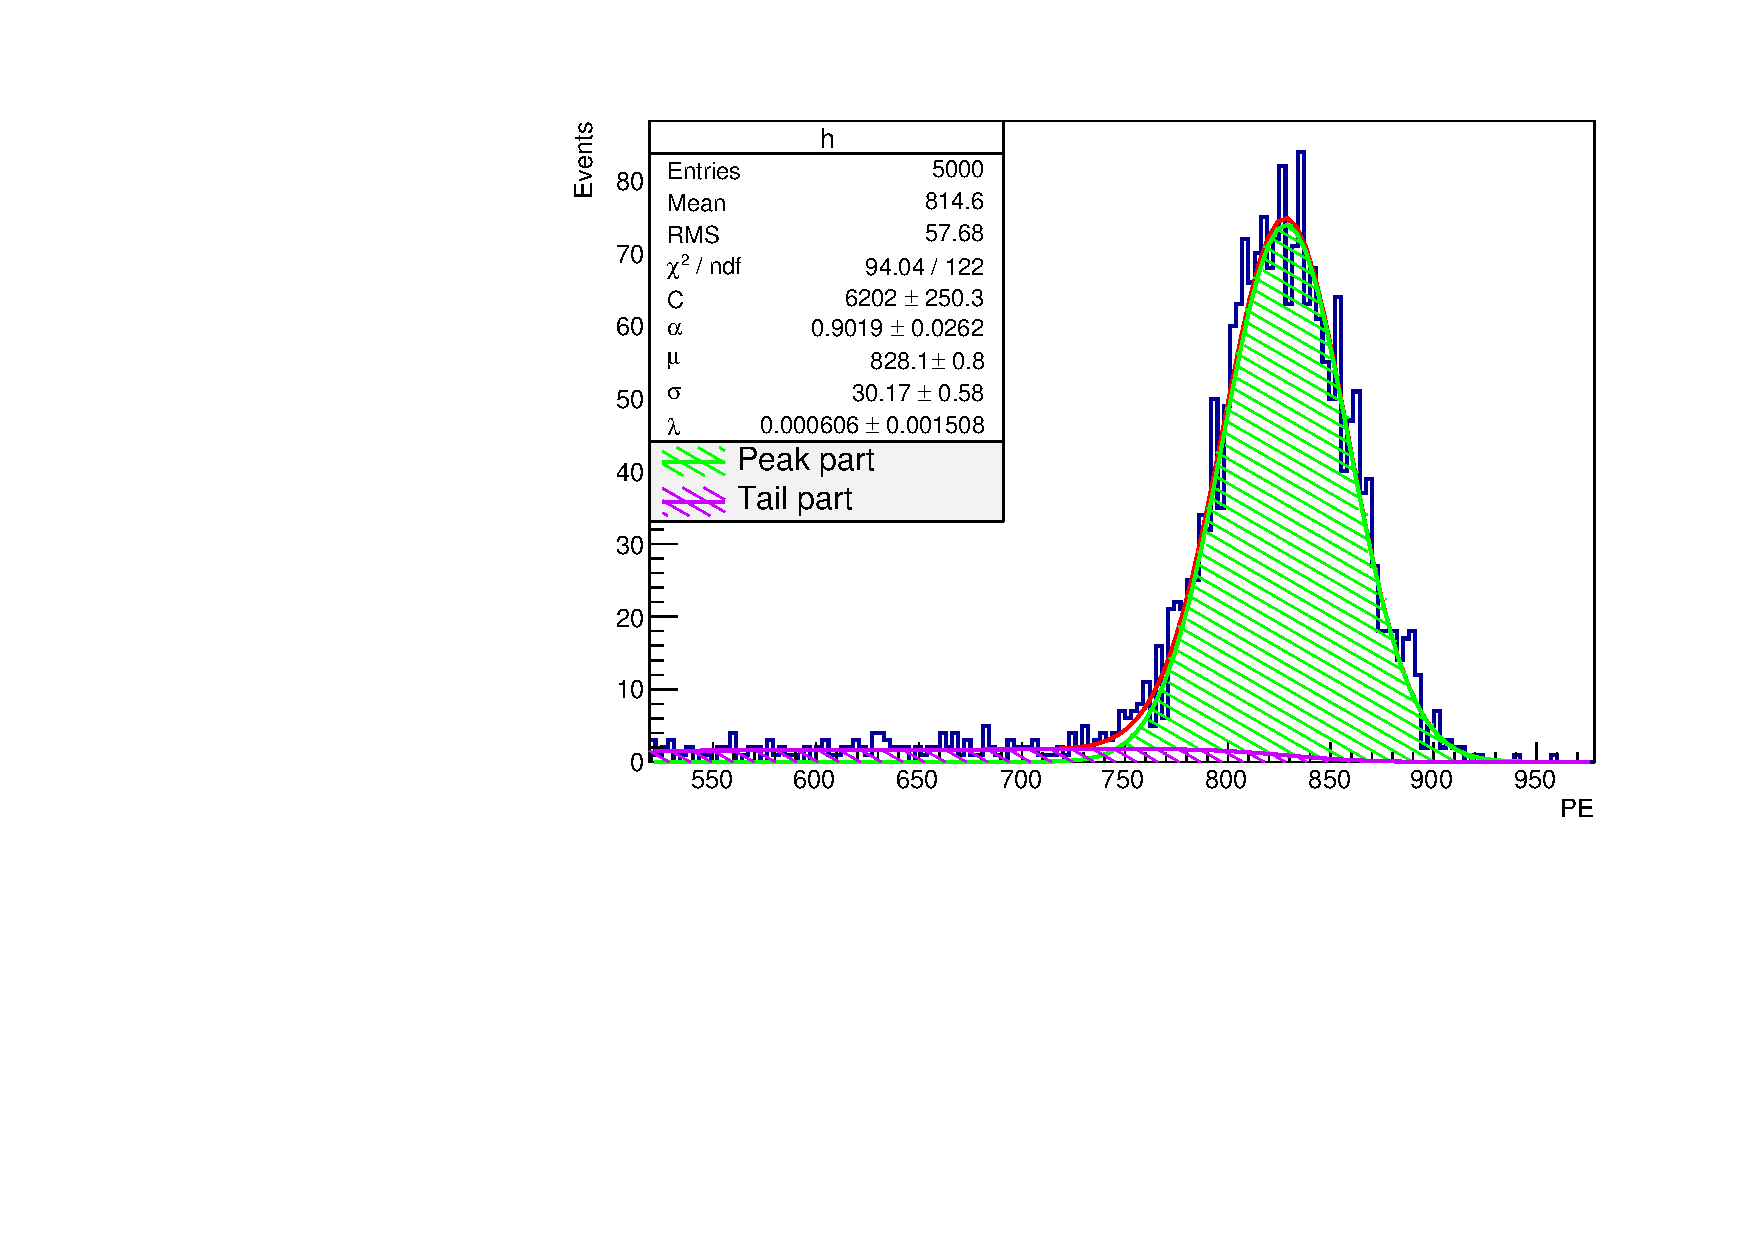
\includegraphics[width=3in]{Cs137.pdf}
	\figcaption{PE spectrum of Cs137 with source enclosure at CD center}
	\label{Cs137}
\end{center}

\begin{center}
	\centering
	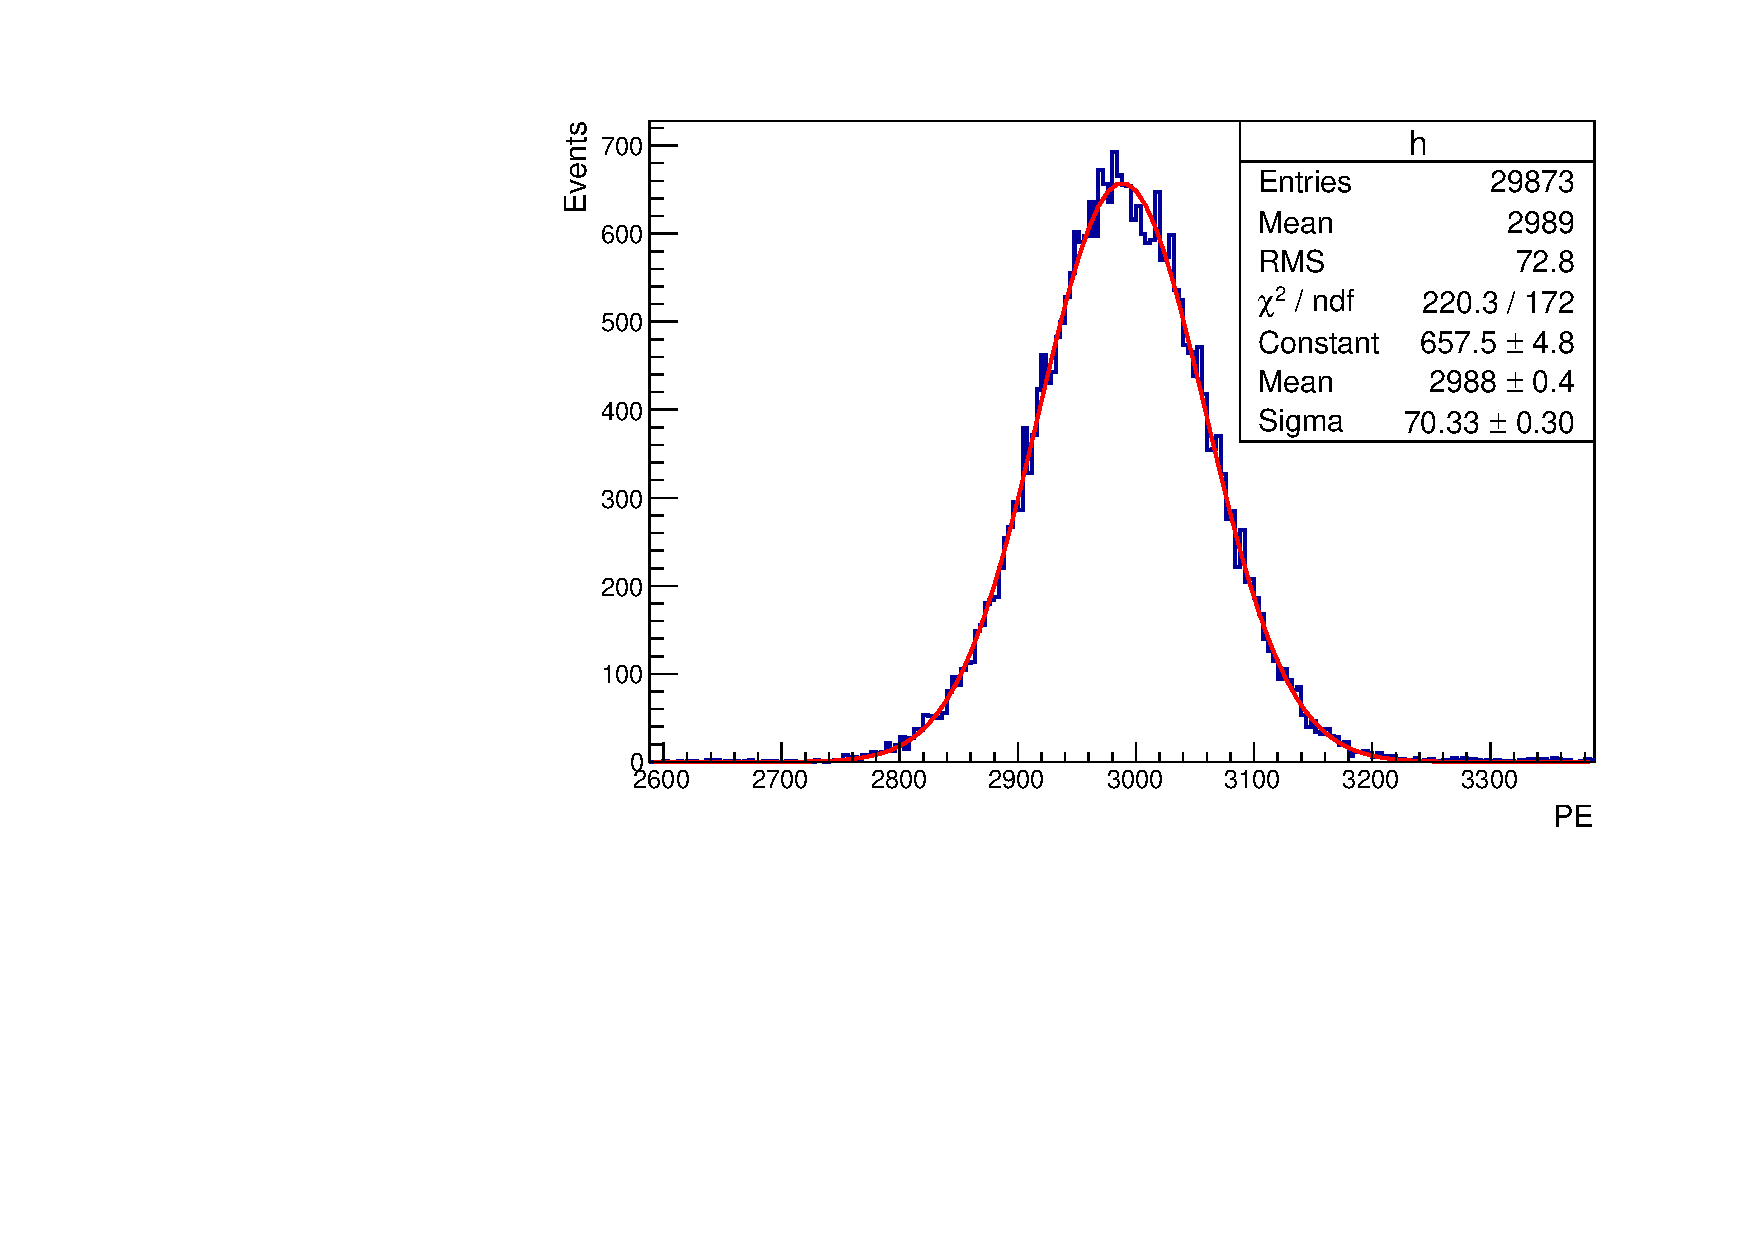
\includegraphics[width=3in]{neutron.pdf}
	\figcaption{The neutron source with source enclosure at CD center}
	\label{neutron}
\end{center}

\begin{center}
	\centering
	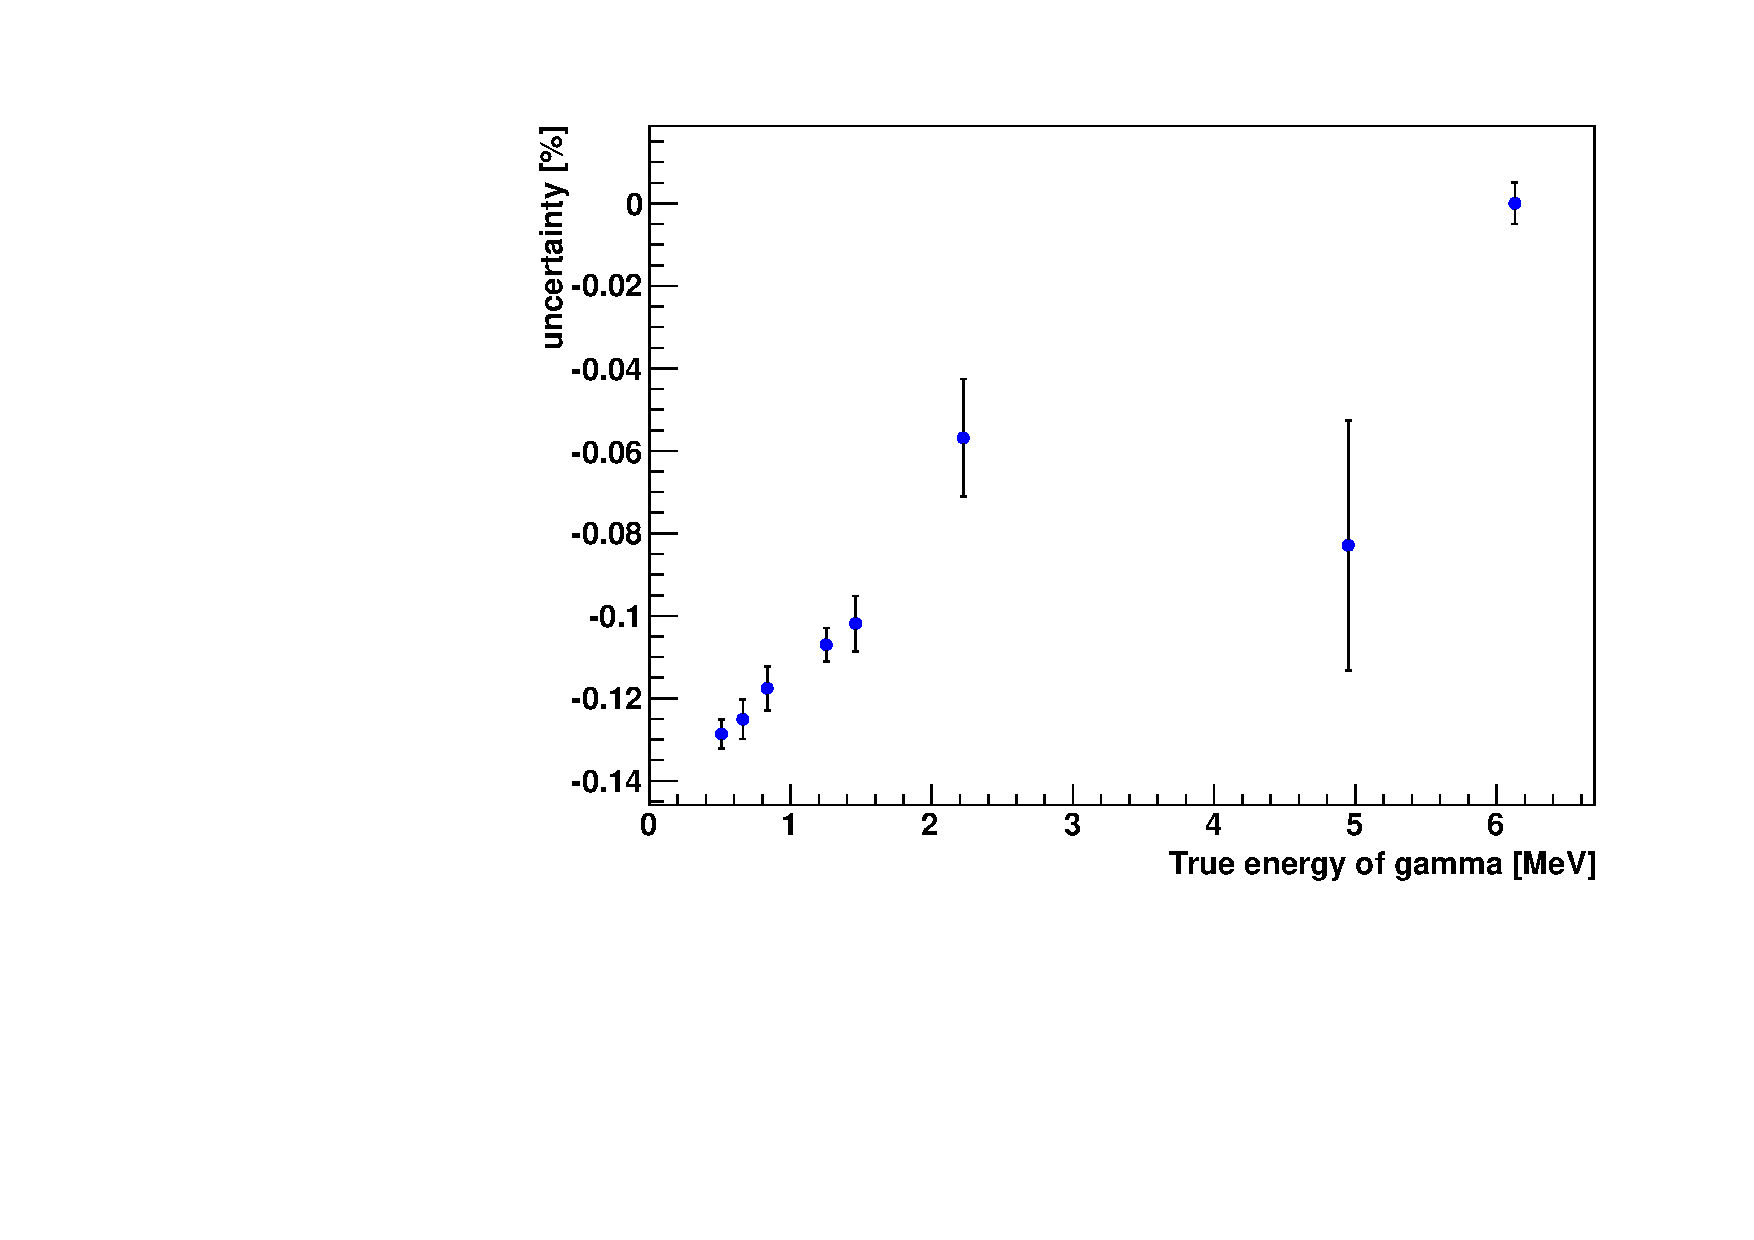
\includegraphics[width=3in]{shadowing_uncertainty.pdf}
	\figcaption{optical shadowing effect}
	\label{shadowing}
\end{center}

\begin{center}
	\centering
	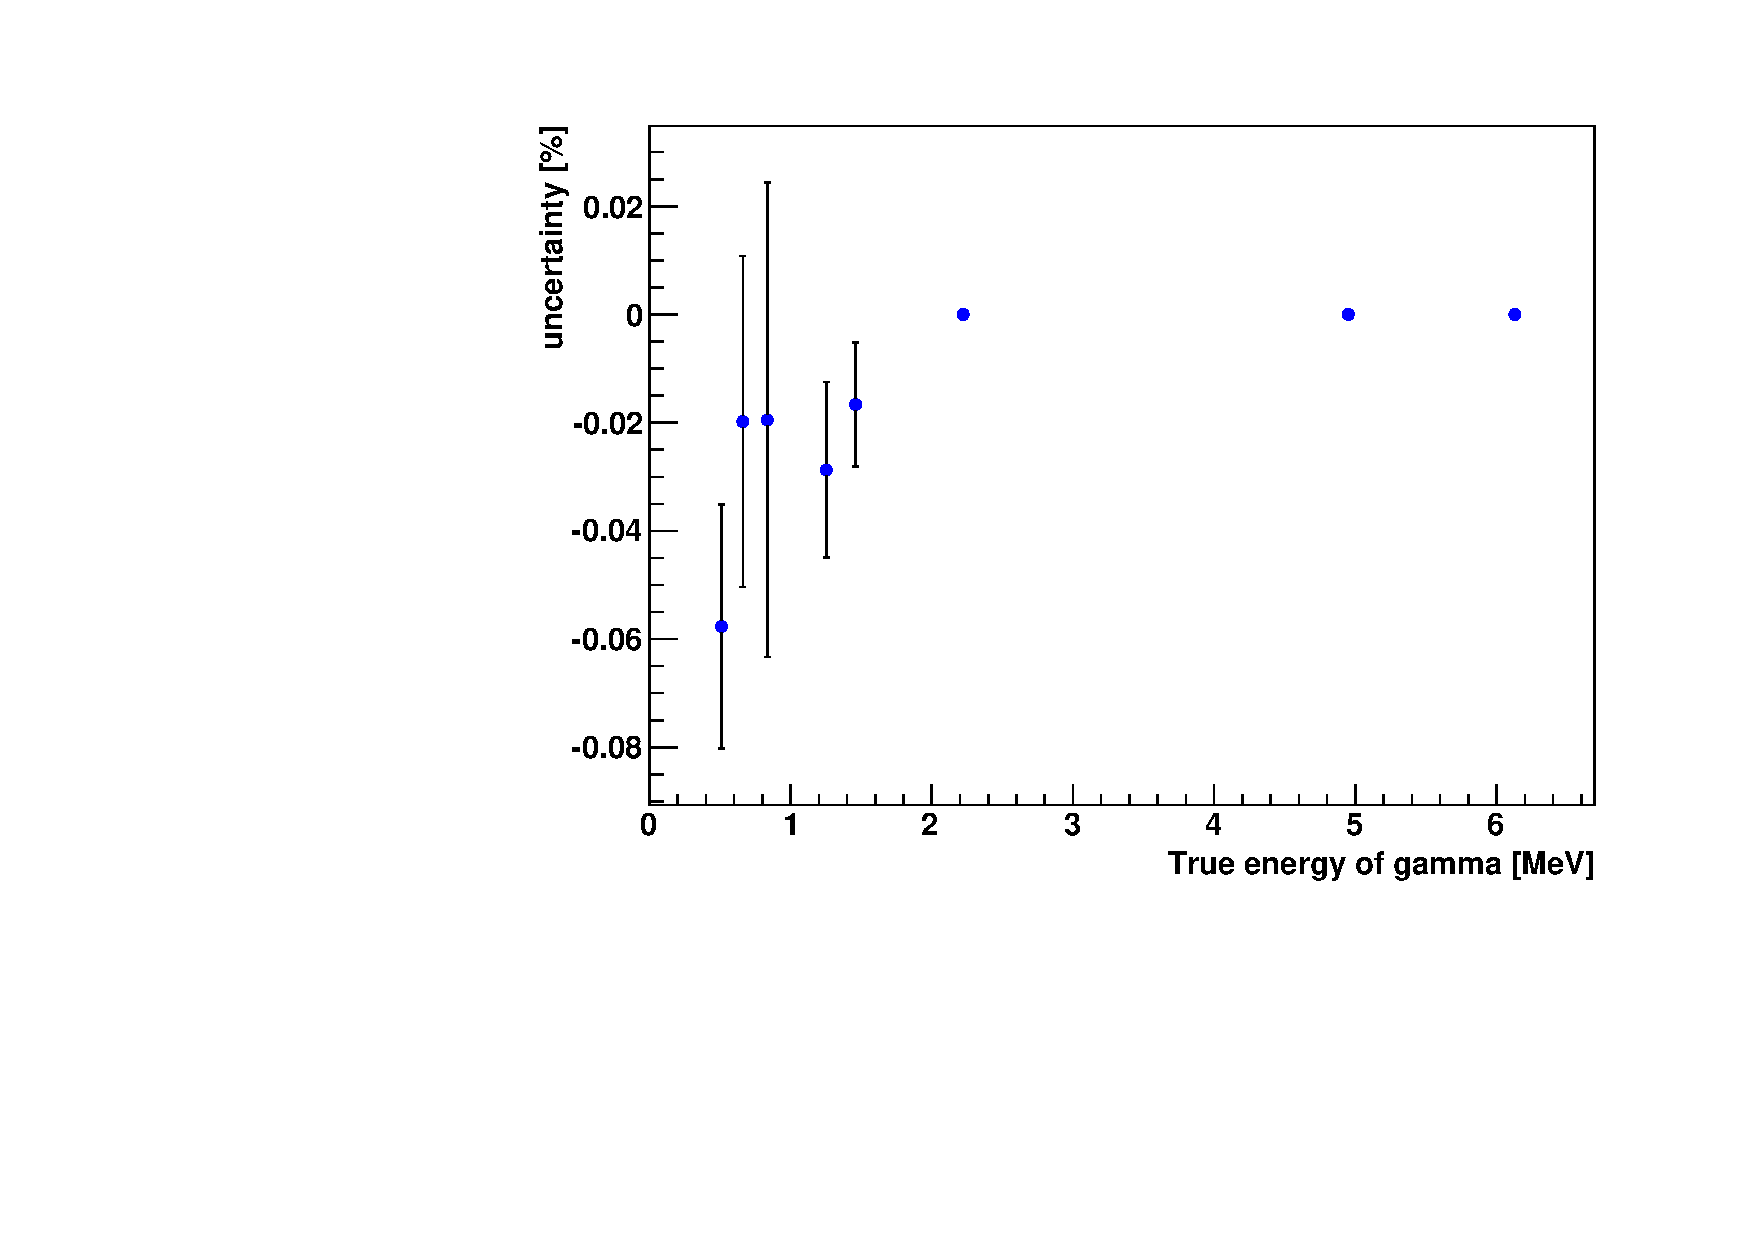
\includegraphics[width=3in]{compton_uncertainty.pdf}
	\figcaption{Compton effect}
	\label{compton}
\end{center}

\section{Control energy uncertainty}
\subsection{Shadowing effect}
The material of source container shell is Teflon. Even the reflectivity is very high (assume 90\% reflectivity in the simulation), there still must be some optical photon loss. So we need to study the shadowing effect. To decouple the shadowing effect and Compton effect, we can select the events without energy loss during the simulation. With the cut, the PE spectrum follows the Gaussian distribution, so we fit it with Gaussian function to obtain mean value as shown in Fig.~\ref{Cs137}. And then compare it with the ideal case, bare source without enclosure. Fig.~\ref{shadowing} shows the uncertainty due to the shadowing effect.
\subsection{Compton effect}
The Compton effect is due to energy loss in non-LS material, and this will introduce Compton shoulder in PE spectrum. And the Compton shoulder will shift the mean value. Even we use the special function to correct this effect, there is still some residual bias. Fig.~\ref{compton} the uncertain due to the Compton effect.
\subsection{Electronic effect}
The non-linearity of electronic can be corrected to 0.3\% uncertainty level with laser calibration system. Here we assume the residual non-linearity is energy dependent, 
\begin{eqnarray}
\label{eq0}
\frac{E_{rec}}{E_{vis}} = 1 + 0.3\%e^{-E_{vis}/t}
\end{eqnarray}
where t = 2.55 MeV


\subsection{Statistical effect}
Assume the rate of source is about 100 Hz. And it will take 5 minutes for every calibration points.
So the total number of events is about 30000. Then we can estimate the uncertainty due to statistic as shown in Fig.~\ref{statistical}. The uncertainty of statistic is energy dependent.
\begin{center}
	\centering
	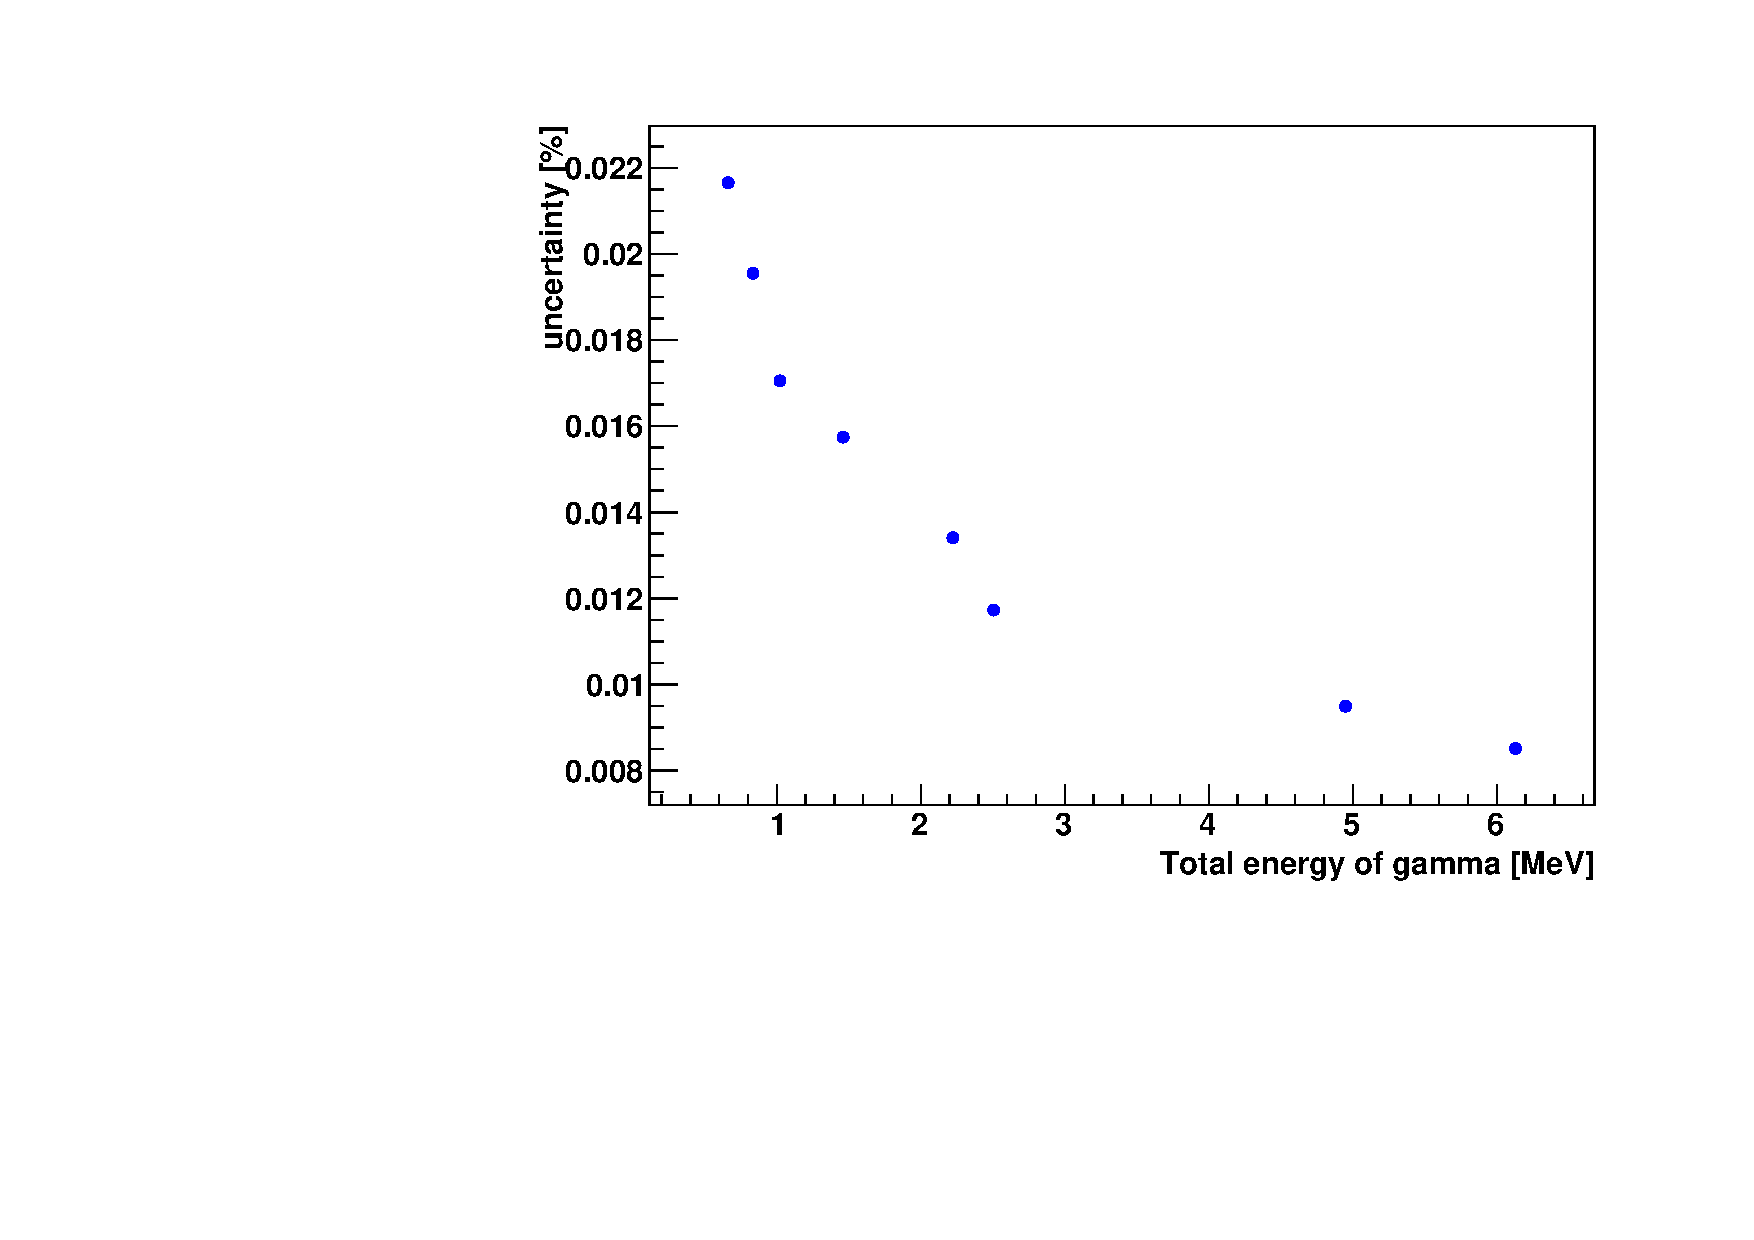
\includegraphics[width=3in]{stat_uncertainty.pdf}
	\figcaption{uncertainty due to the statistic}
	\label{statistical}
\end{center}

\section{Energy scale}
One of main purpose of JUNO calibration is to make uncertainty of the scale less than 1\%. In order to reach this physics requirement, we should have a better understanding of the energy non-linearity of detector response. A series of radioactive sources will be used to do the calibration of energy non-linearity, including gamma sources, neutron source and beta source. 

\subsection{Energy non-linearity of gamma}
Here we will introduce the strategy of JUNO calibration based on MC simulation result. The full absorption peak of delay signal of neutron capture at Hydrogen (2.22 MeV) is determined as the energy scale. Then we can reconstruct energy of other calibration source with PE/scale. The reconstructed energy is different from true energy due to energy non-linearity. The ratio of reconstructed energy and true energy will be described as energy dependent of non-linearity. Fig.~\ref{non_linearity_fit} shows the energy non-linearity of gamma from 0.511 MeV to 6.13 MeV, which can be obtained from calibration system.

\begin{center}
	\centering
	%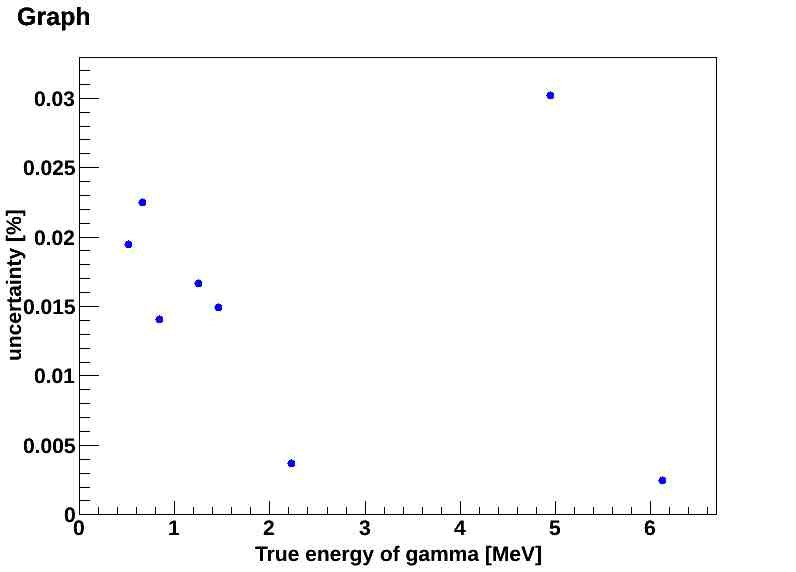
\includegraphics[width=3in]{statistical.jpg}
	%\subfigure[]{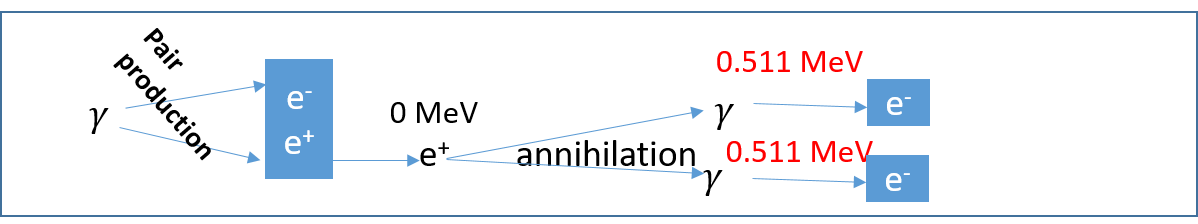
\includegraphics[width=4in]{gamma2e_1.png}}
	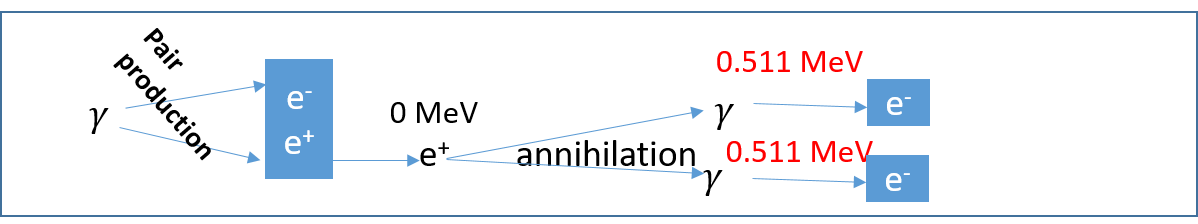
\includegraphics[width=3in]{gamma2e_1.png}
	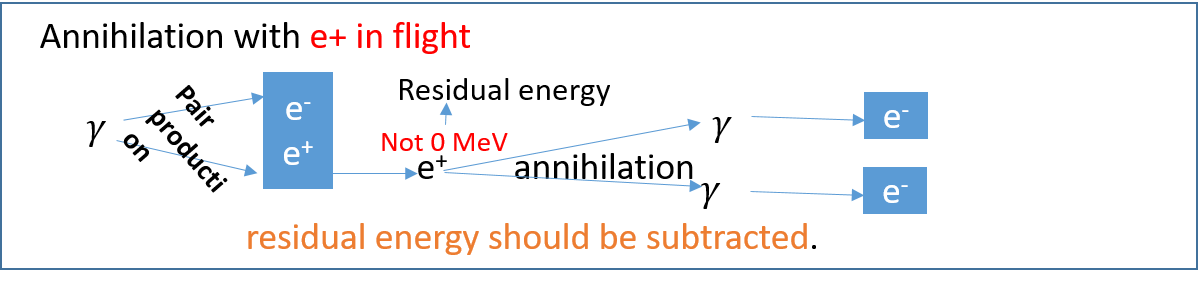
\includegraphics[width=3in]{gamma2e_2.png}
	%\subfigure[]{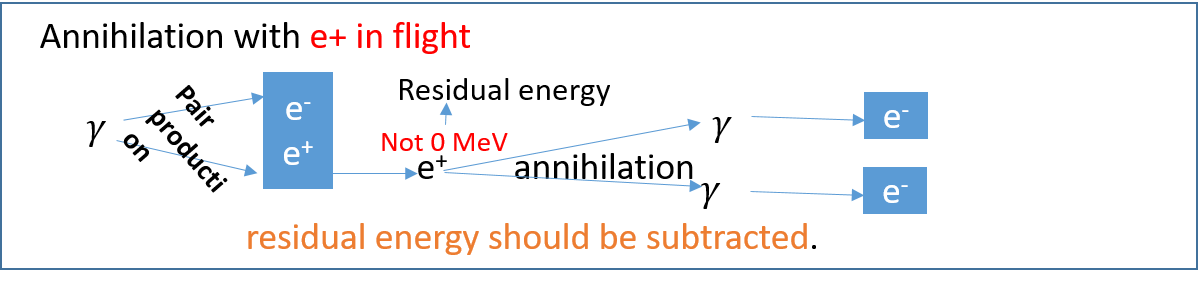
\includegraphics[width=4in]{gamma2e_2.png}}
	\figcaption{The relationship between gamma and electron}
	\label{gamma2e}
\end{center}

\begin{center}
	\centering
	%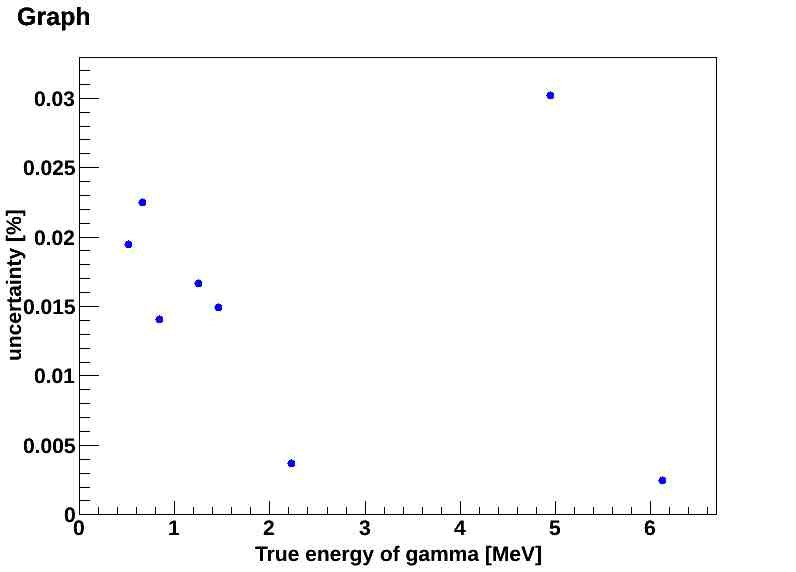
\includegraphics[width=3in]{statistical.jpg}
	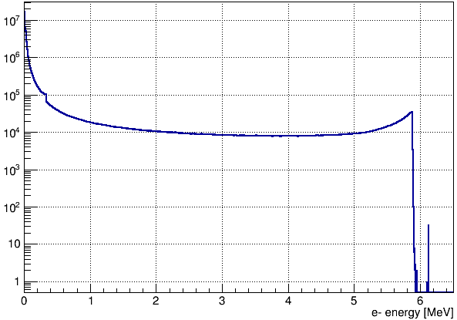
\includegraphics[width=2in]{gamma_e_pdf1.png}
	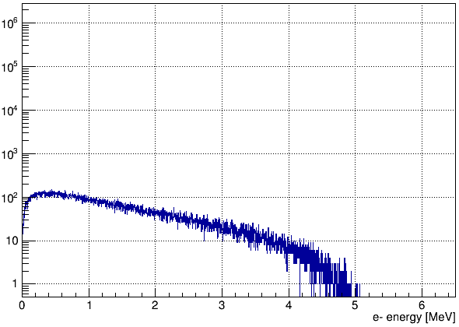
\includegraphics[width=2in]{gamma_e_pdf2.png}
	\figcaption{Probability of energy density function of electron from gamma}
	\label{gamma_e_pdf}
\end{center}


\subsection{Relationship between gamma and electron}
However, IBD events is positron events. So we would like to know the response of positron energy non-linearity. The relation between gamma and electron can be established with Geant4. And we assume that electron and positron have almost same action of energy non-linearity in addition to two gammas from positron annihilation.  There are mainly three physics process for the conversion from gamma to electron, including pair production, Compton scattering, photoelectric effect, as shown in Fig.~\ref{gamma2e}. Fig.~\ref{gamma_e_pdf} shows the probability density function (PDF) of energy of electron with initial energy of gamma 6.13 MeV.  

\subsection{Model of energy non-linearity}
Referring to Daya Bay's method, an empirical formula with 4 parameters was used to describe energy non-linearity of electron, 
\begin{eqnarray}
\label{eq1}
\frac{E_{vis}}{E_{true}} = \frac{P_{0}+P_{3}E_{true}}{1+P_{1}e^{-P_{2}E_{true}}}. 
\end{eqnarray}

The energy non-linearity of gamma can be deduced with both the empirical formula and the PDF of electron energy.

\begin{center}
	\centering
	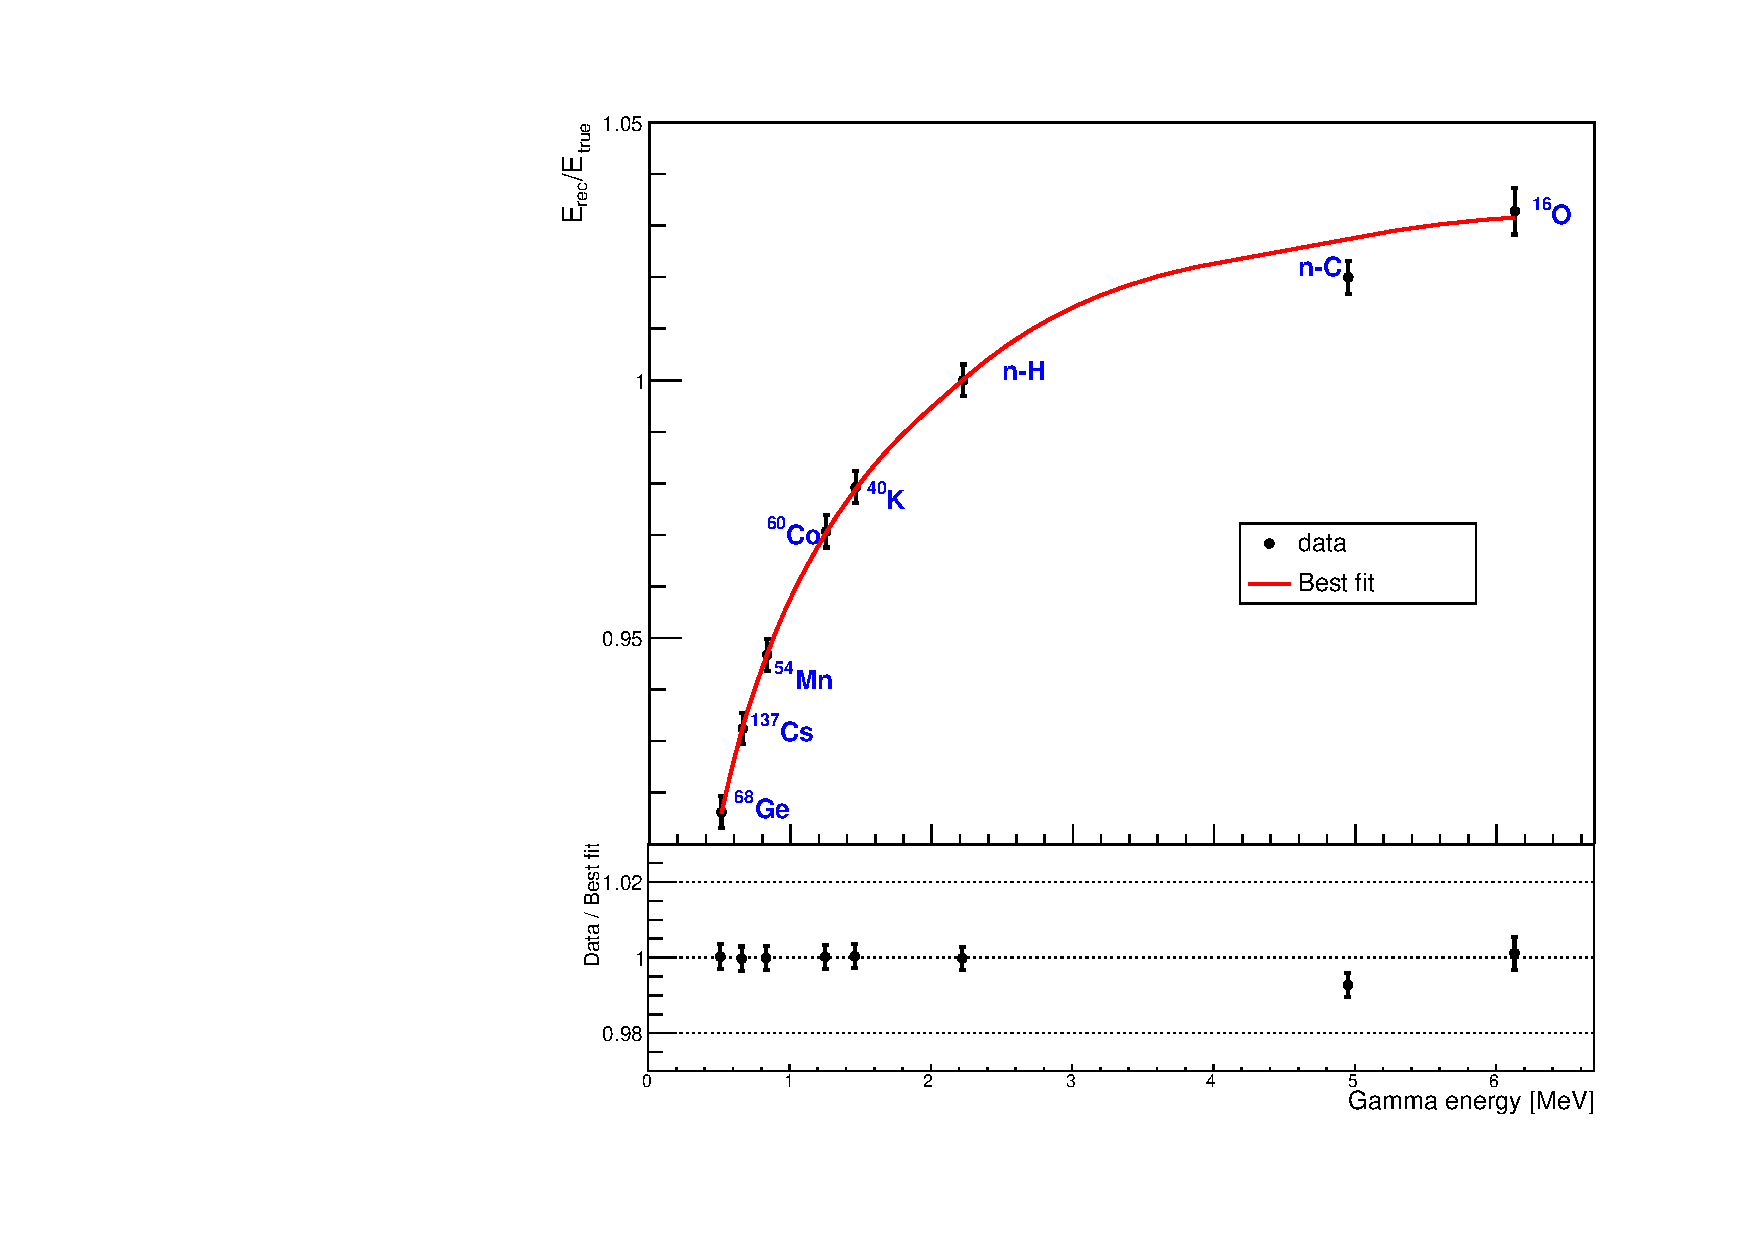
\includegraphics[width=3in]{non_linearity_fit.pdf}
	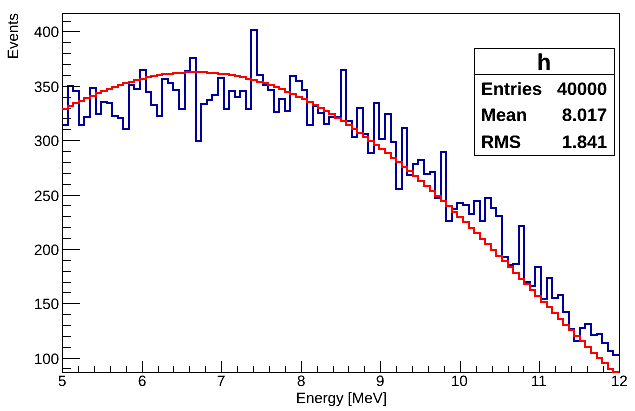
\includegraphics[width=2.7in]{B12.png}
	\figcaption{Fit to data with Eq.~(\ref{eq1})}
	\label{non_linearity_fit}
\end{center}



\begin{center}
	\centering
	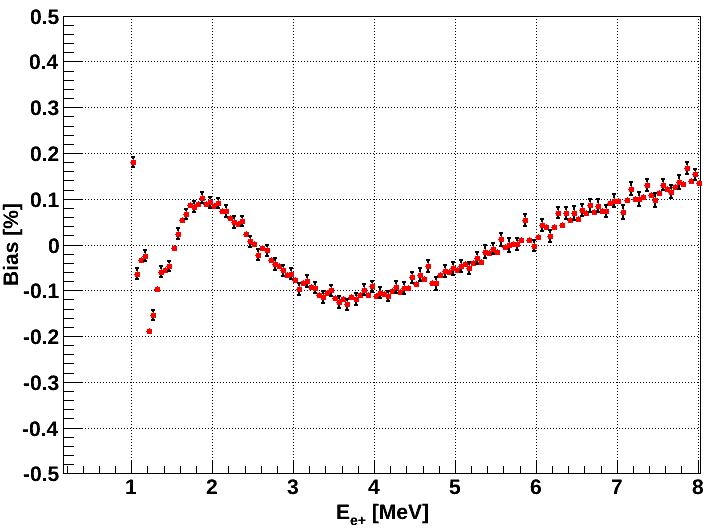
\includegraphics[width=2.5in]{bias_positron.png}
	\figcaption{bias of positron non-linearity after correction}
	\label{bias_positron}
\end{center}

\subsection{Energy non-linearity of positron}
The data of gamma energy non-linearity can be obtained from calibration. With the model we have established, we can fit the data to extract the parameters. Then we get the non-linearity of electron. The only different between electron and positron is annihilation gamma. And this effect can be calibrated with Ge68, ignoring annihilation in flight. The Fig.~\ref{non_linearity_fit} shows the result of fitting with the model of energy non-linearity.

\begin{center}
	\centering
	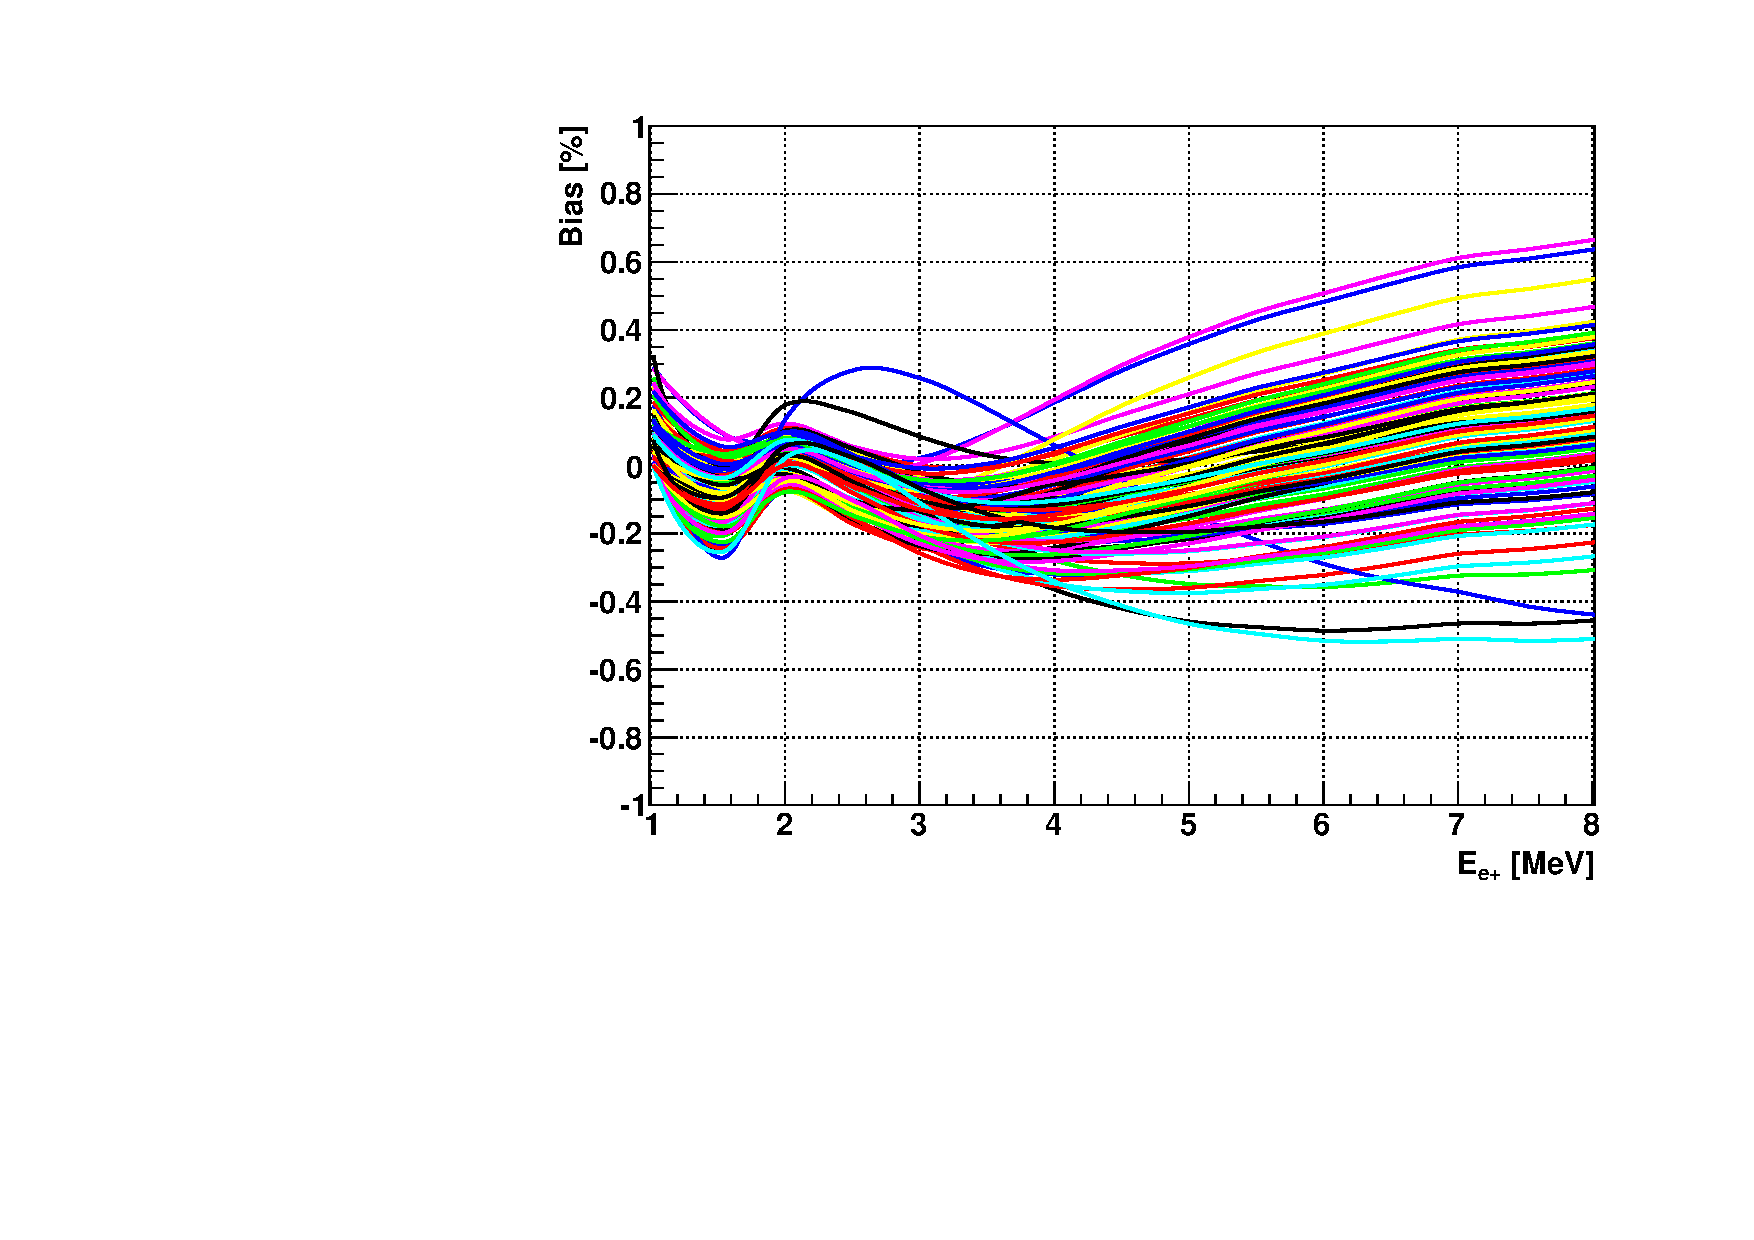
\includegraphics[width=3in]{sys_uncertainty_non-linearity.pdf}
	\figcaption{Systematic uncertainty analysis}
	\label{sys_uncertainty_non-linearity}
\end{center}

\subsection{Systematic uncertainty analysis}
Then we consider the uncertainty from optical shadowing effect, Compton tail, statistic effect and electronic non-linearity effect.
Assuming we cannot get exact mean for every calibration source, every source will be randomly added bias based on the uncertainty. Then we can get the corresponding bias of positron non-linearity. And repeat this procedure multiple times. For every time, we get one curve for the bias. 
The overall bias is shown in Fig.~\ref{sys_uncertainty_non-linearity}
\section{Energy resolution}

\begin{center}
	\centering
	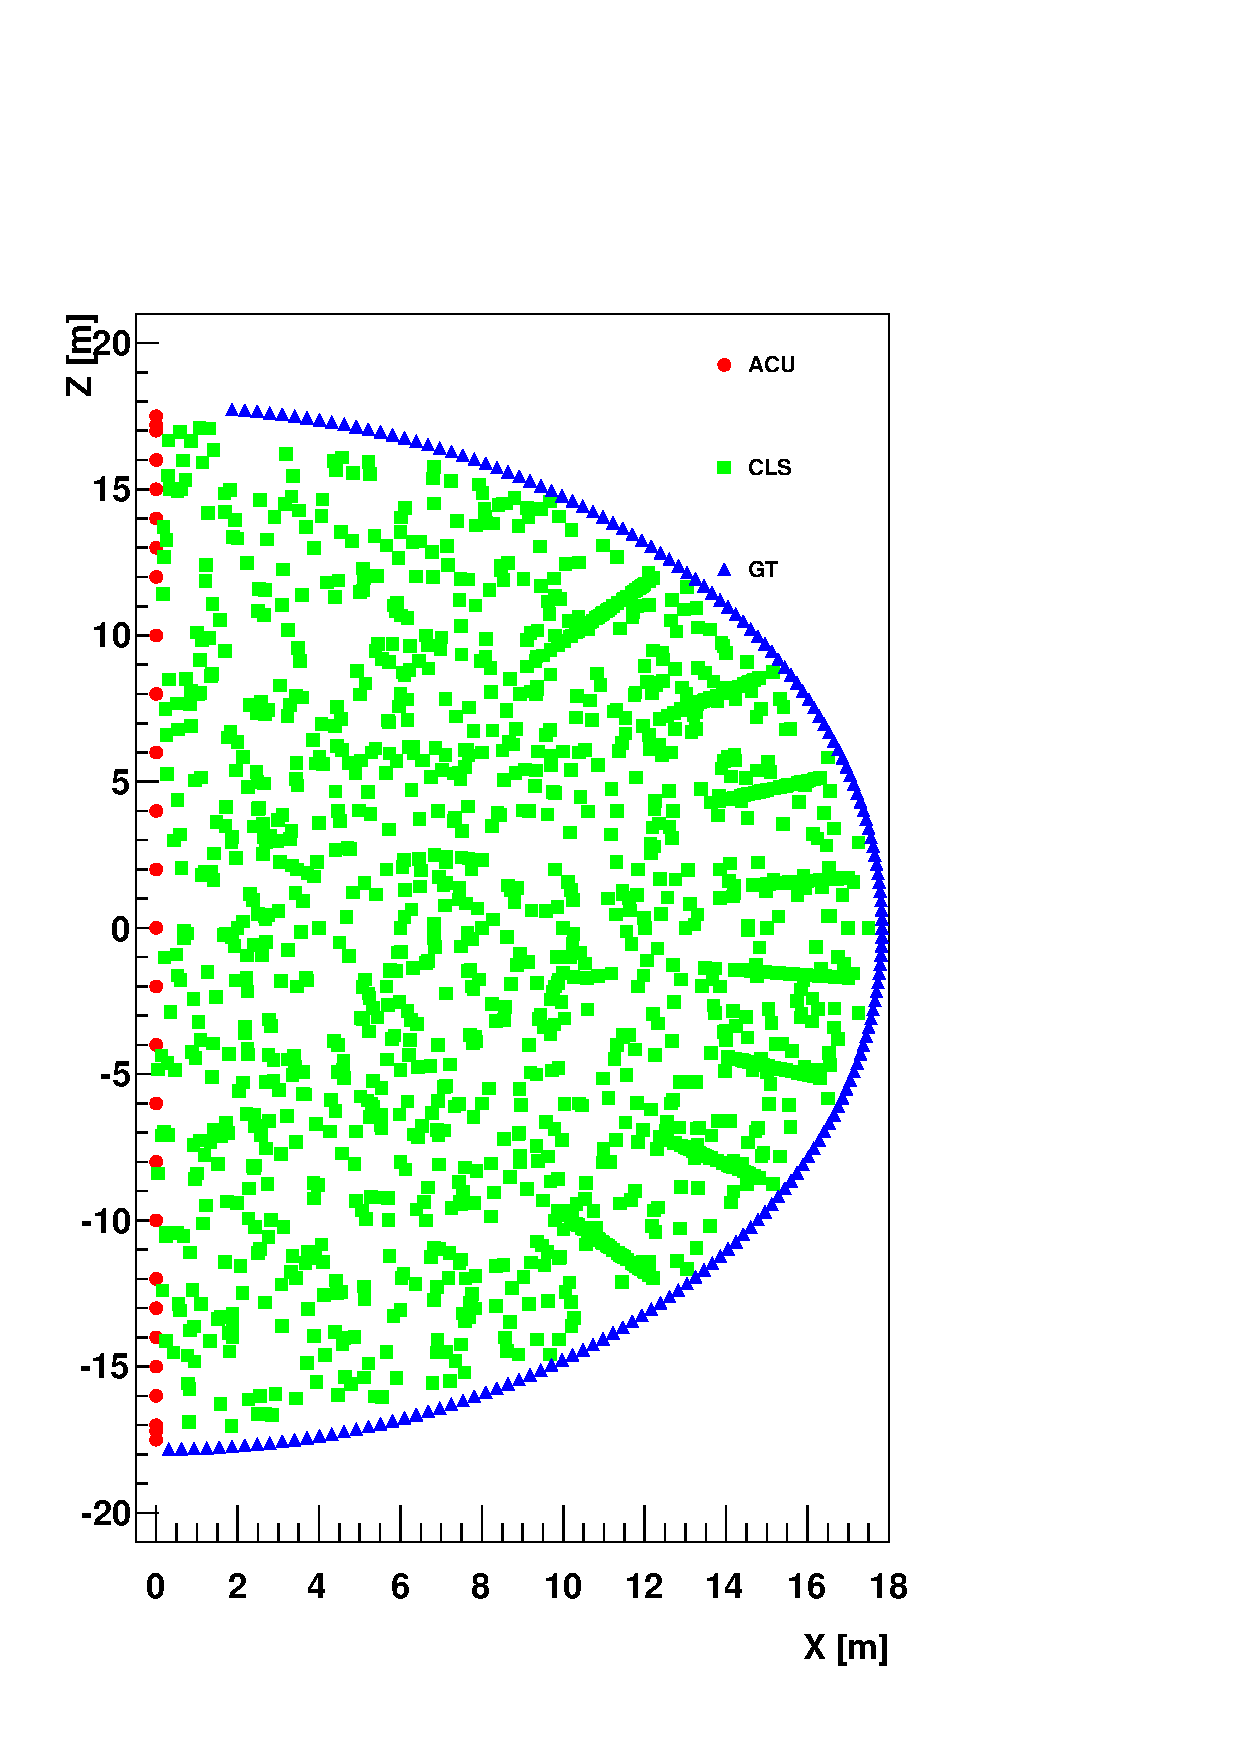
\includegraphics[width=3in]{calibration_mapping.pdf}
	\figcaption{calibration mapping}
	\label{calibration_mapping}
\end{center}

\begin{center}
	\centering
	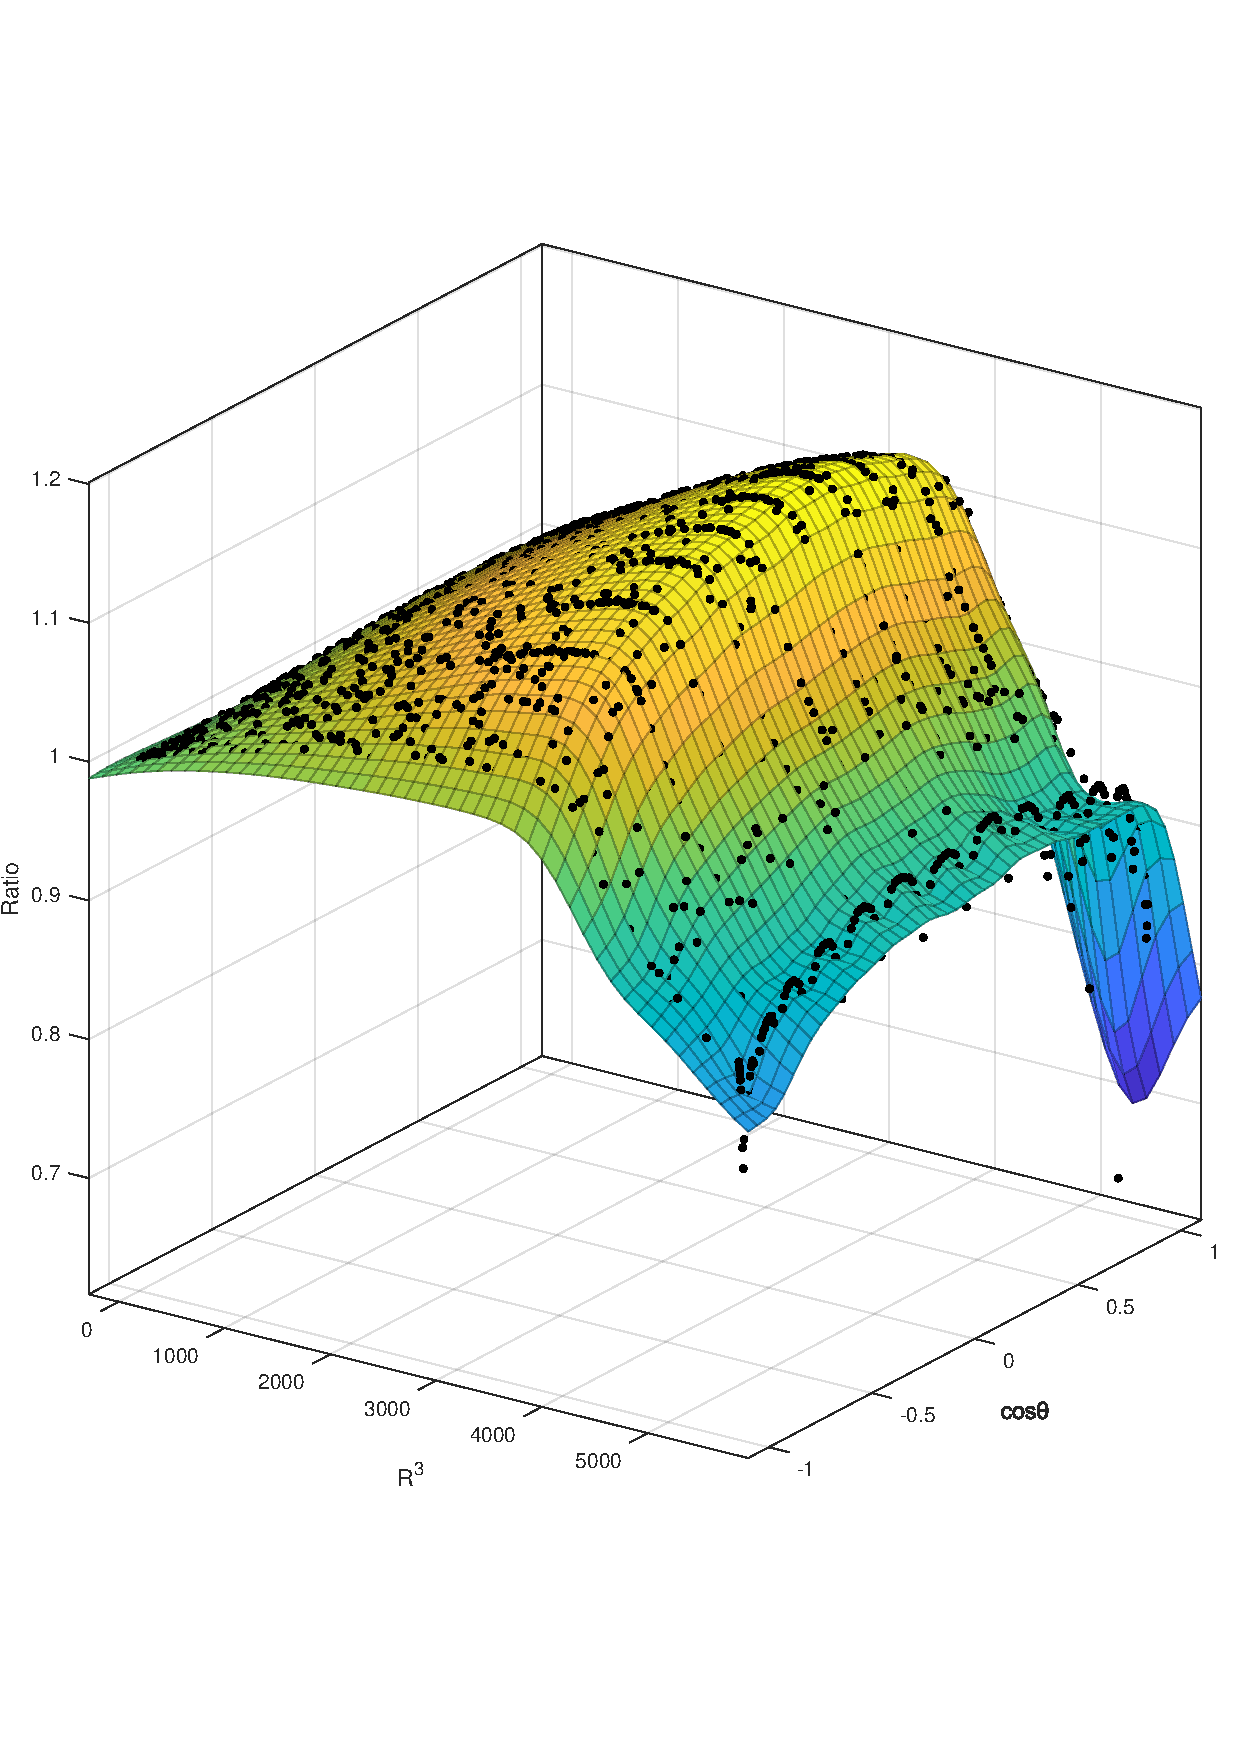
\includegraphics[width=3in]{spline_function.pdf}
	\figcaption{spline function}
	\label{spline_function}
\end{center}

\begin{center}
	\centering
	%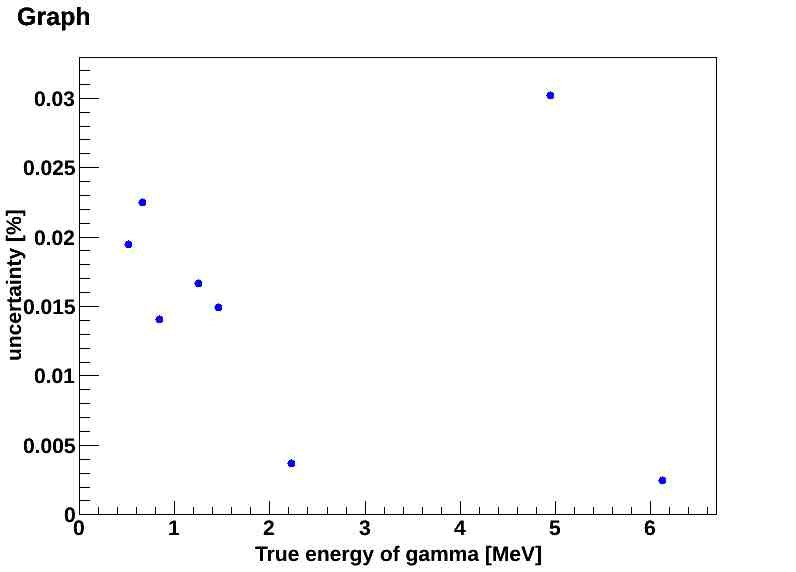
\includegraphics[width=3in]{statistical.jpg}
	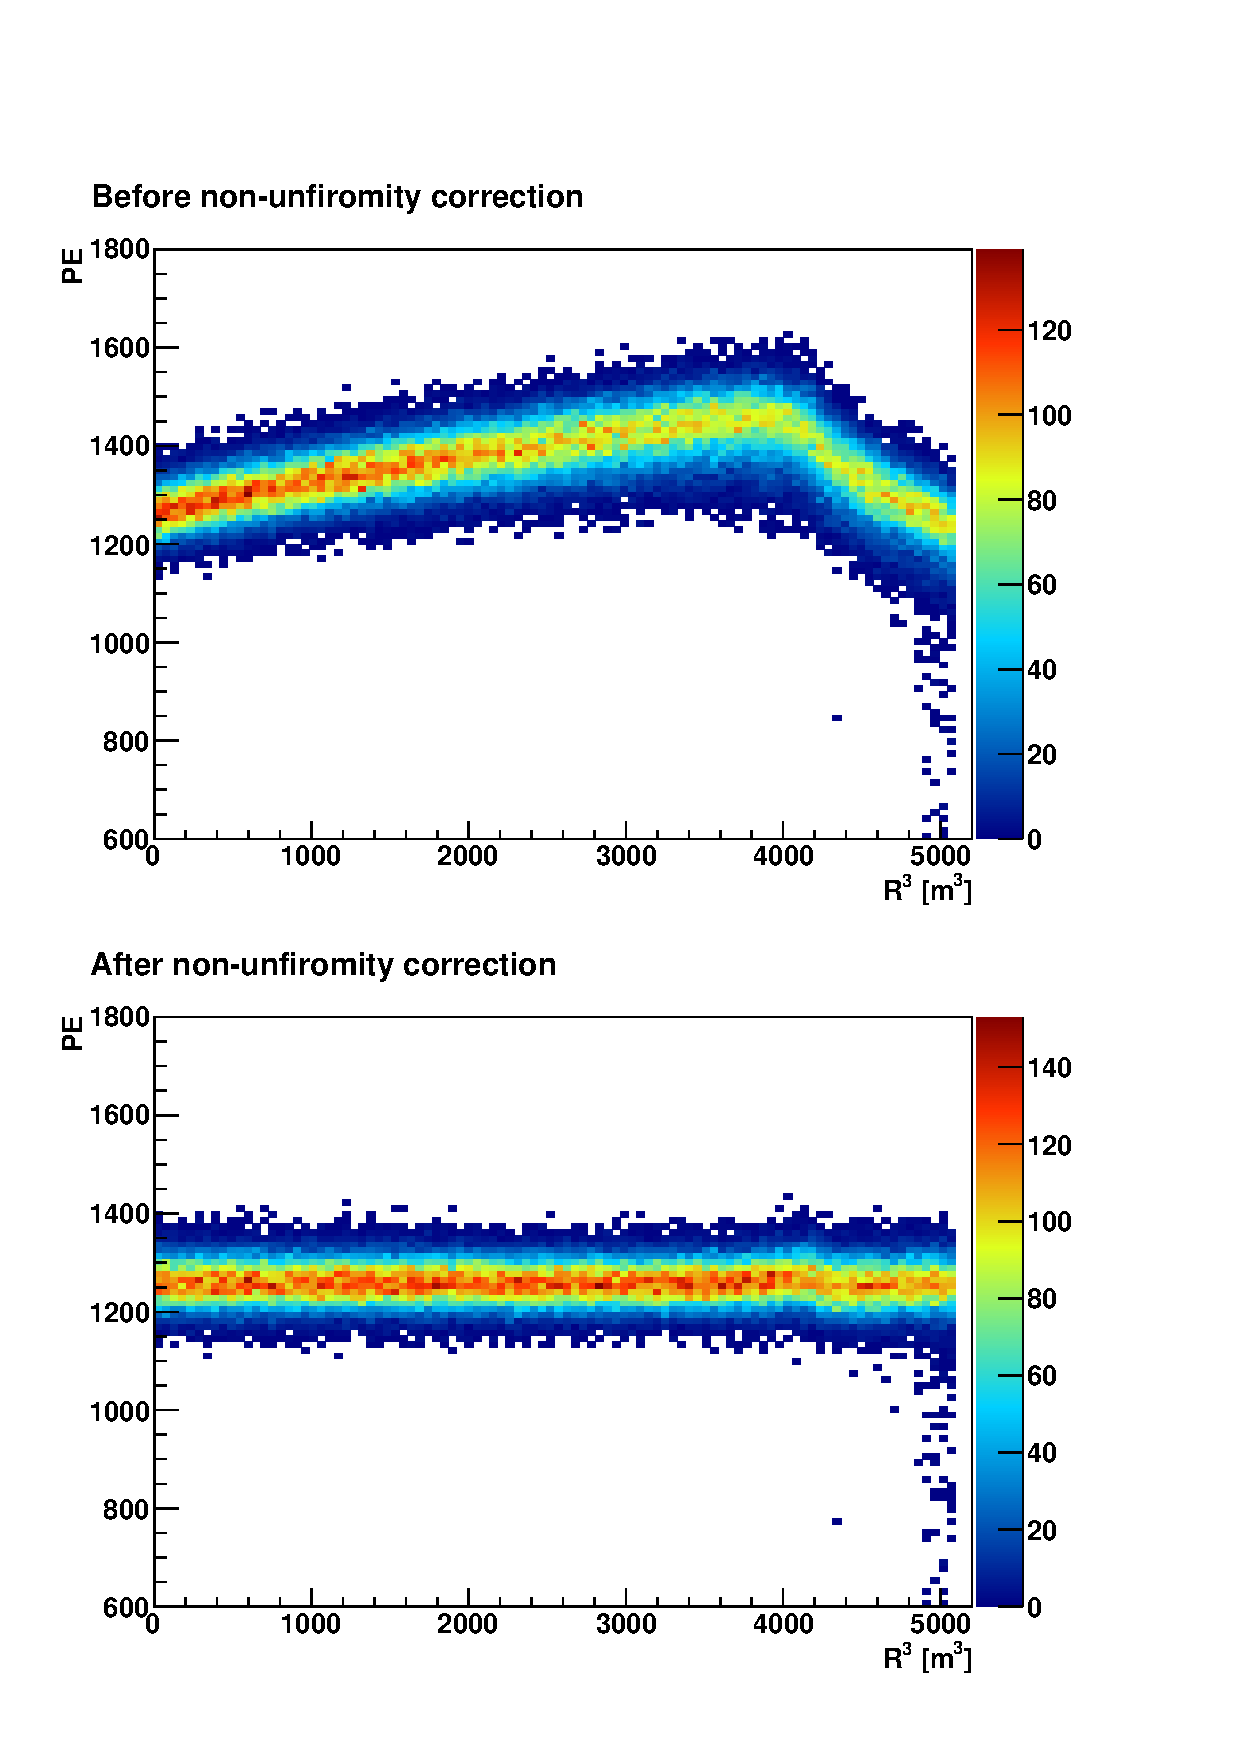
\includegraphics[width=2.5in]{non_uniform_correction.pdf}
	\figcaption{non uniformity correction}
	\label{mono_energy}
\end{center}

With calibration system of CLS, sources can be deployed in one vertical plane. Assuming the response of detector is phi symmetrical, we can do the non-uniformity correction with the vertical calibration mapping. The calibration mapping is shown in Fig.~\ref{calibration_mapping}.  We use one thin plate spline function to fit the data to describe the non-uniformity, as  shown in Fig.~\ref{spline_function}. The function shows the corresponding ratio to CD center. With algorithm of vertex reconstruction, we can get the vertex of IBD events. Then we can correct the non-uniformity by scaling it to CD center. 
Then we do simulation to qualify the non-uniformity. The mono energy positron uniformly generates in CD. Fig.~\ref{mono_energy} a shows the energy spectrum of positron, which shows bad energy resolution. Then with the calibration mapping, we can correct it. Fig.~\ref{mono_energy} b is the energy spectrum after correction, showing better energy resolution with fiducial volume cut R < 17.2 m. We fit the spectrum with Gaussian function to obtain full absorption peak and sigma, then energy resolution can define as sigma/mean. So we use the energy resolution to qualify the non-uniformity correction.

\begin{center}
	\centering
	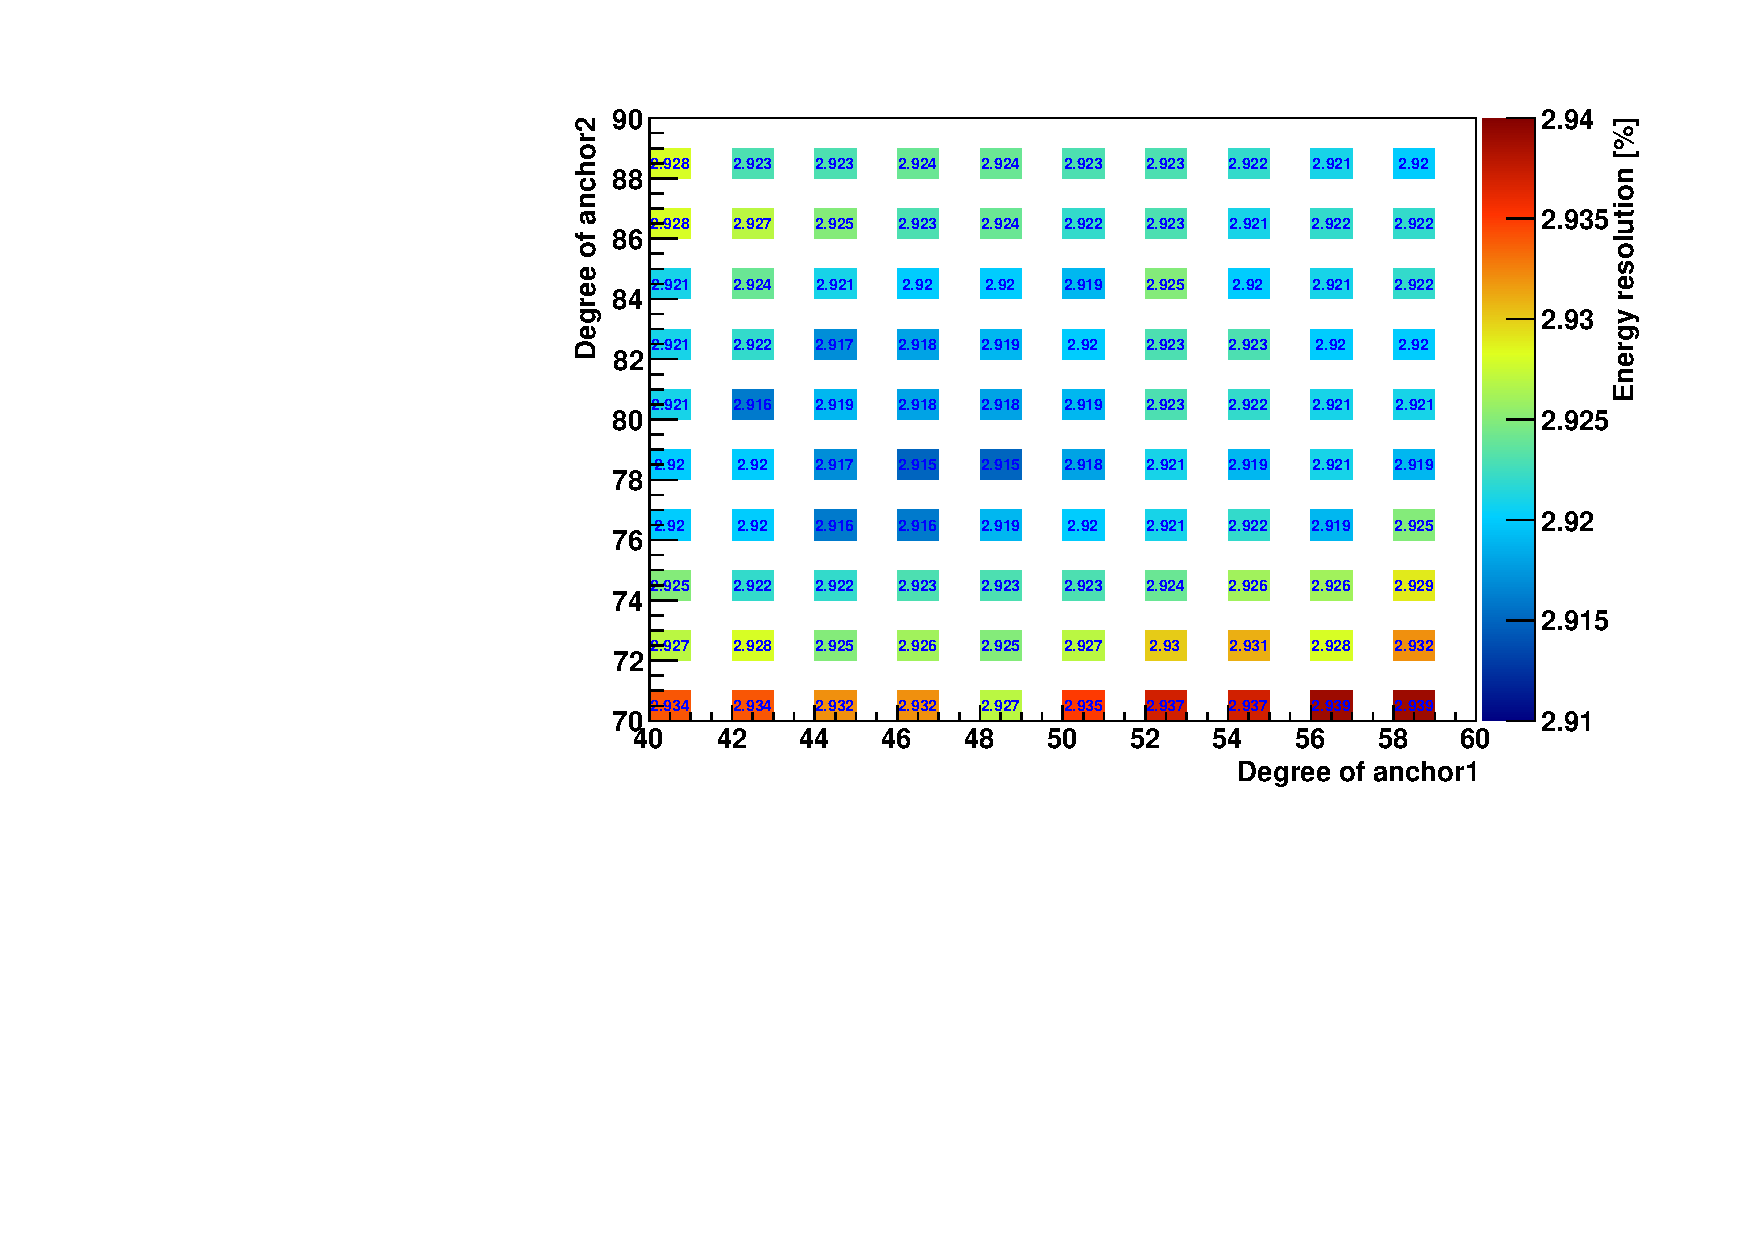
\includegraphics[width=4in]{best_anchor.pdf}
	\figcaption{best anchor position}
	\label{best_anchor}
\end{center}

\subsection{Best CLS anchor determinations.}


In order to maximize scanning area of calibration, we try to use two asymmetrical CLSs to deploy the source. 
Therefore, we need to determine the positions of two anchors. Due to self-weight, the cable is not straight, so the source cannot be deployed to the boundary of detector.
And in this study, 
we naively assume the slope angle of cable is 10 degrees as you can see the figure.
Varying the two anchor position, we construct different calibration mappings. Then calculate the corresponding energy resolution. 
Fig.~\ref{best_anchor} shows the energy resolution as function of anchor positions. From the calculation, we get the best choice of anchor position (48,78) corresponding minimum energy resolution 2.915\%. 

\begin{center}
	\centering
	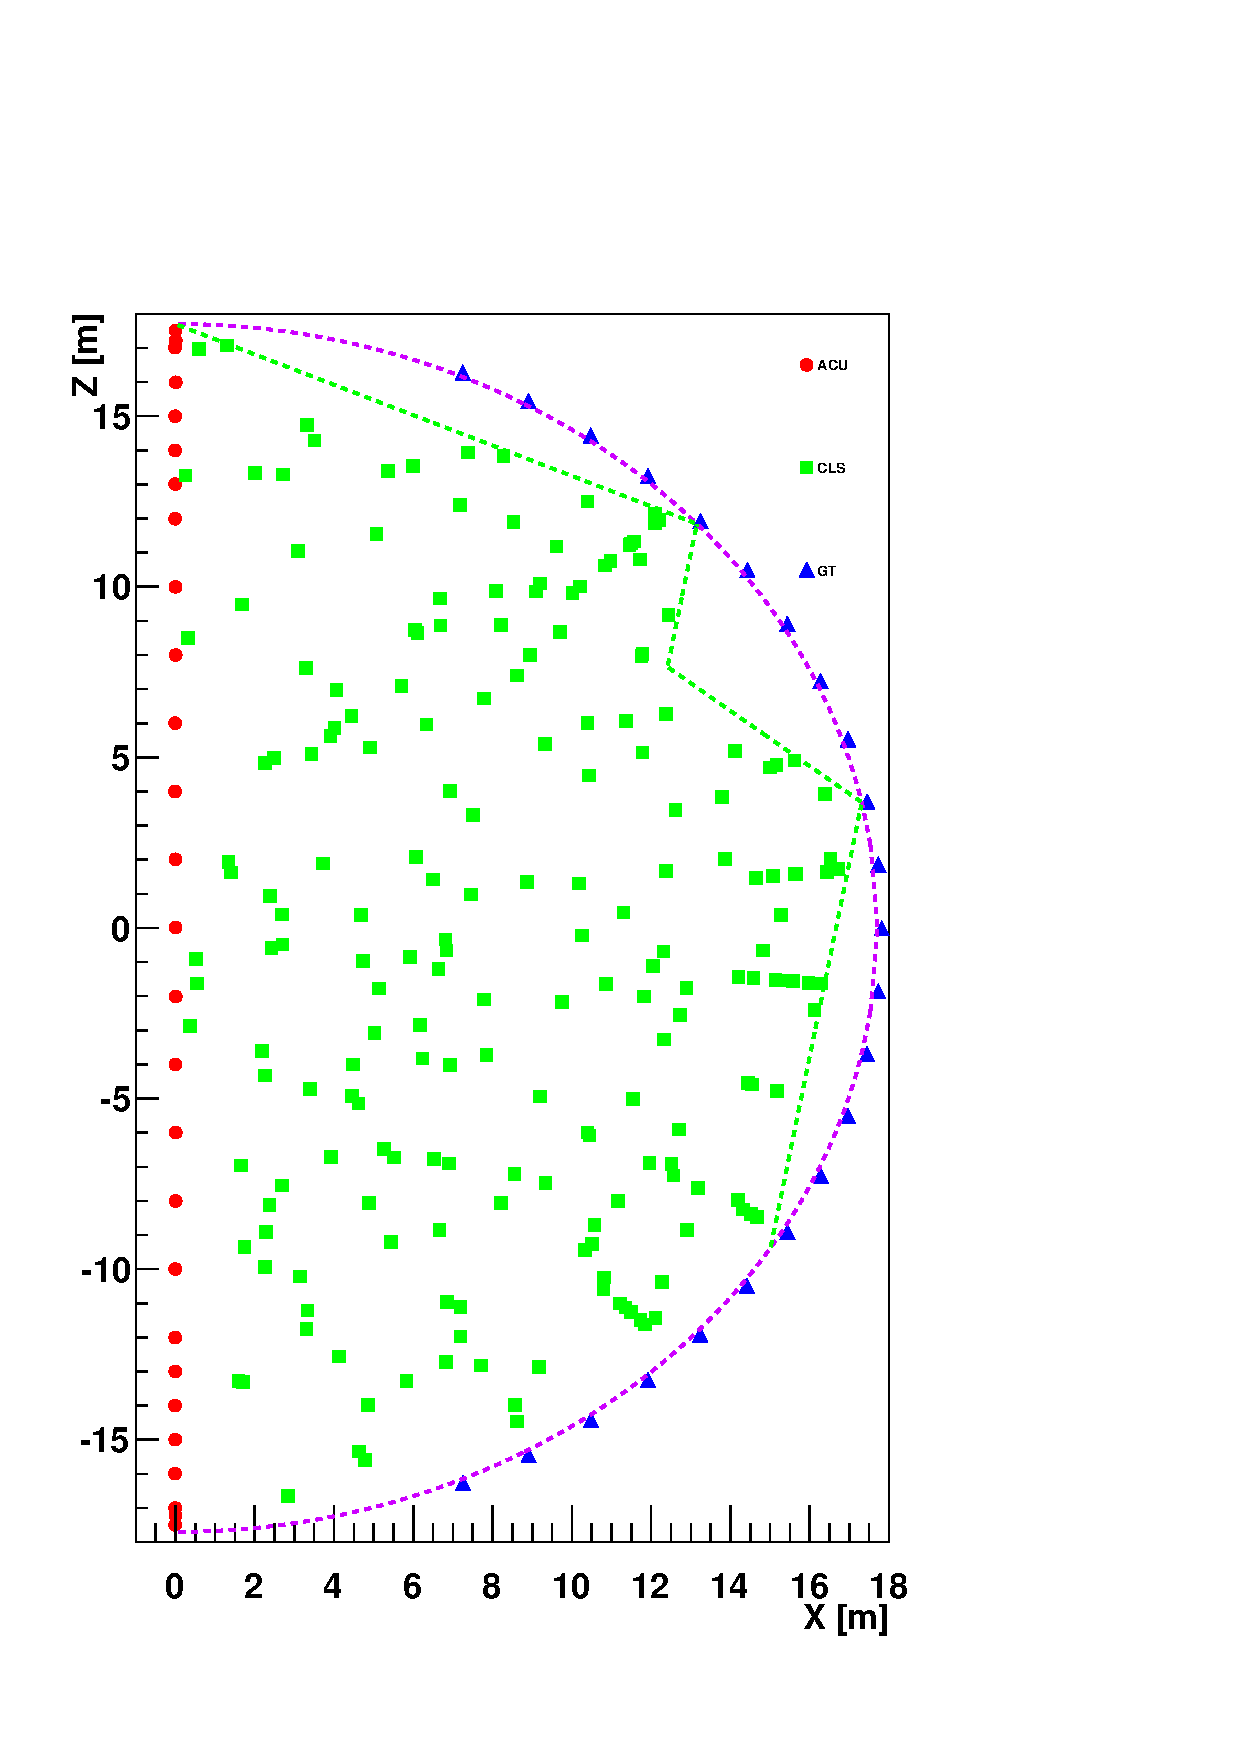
\includegraphics[width=3in]{basic_coverage.pdf}
	\figcaption{basic converage with ACU, CLS and GT}
	\label{basic_coverage}
\end{center}

\begin{center}
	\centering
	%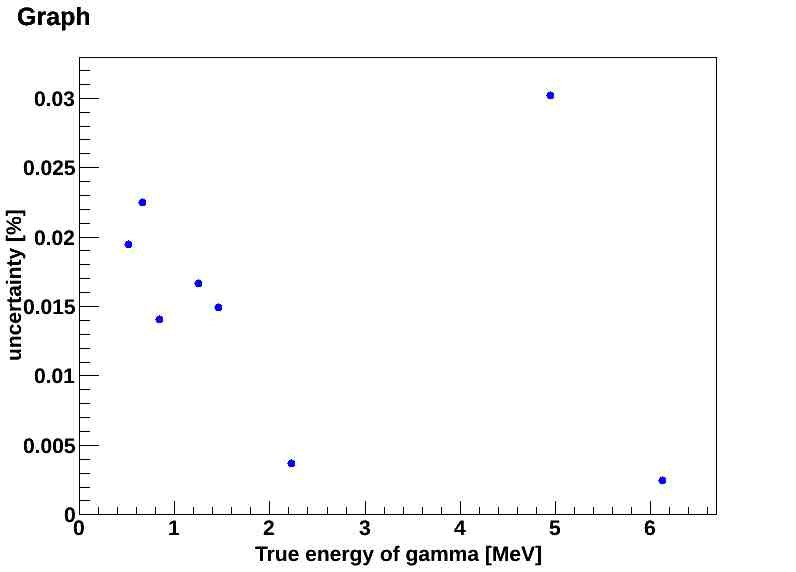
\includegraphics[width=3in]{statistical.jpg}
	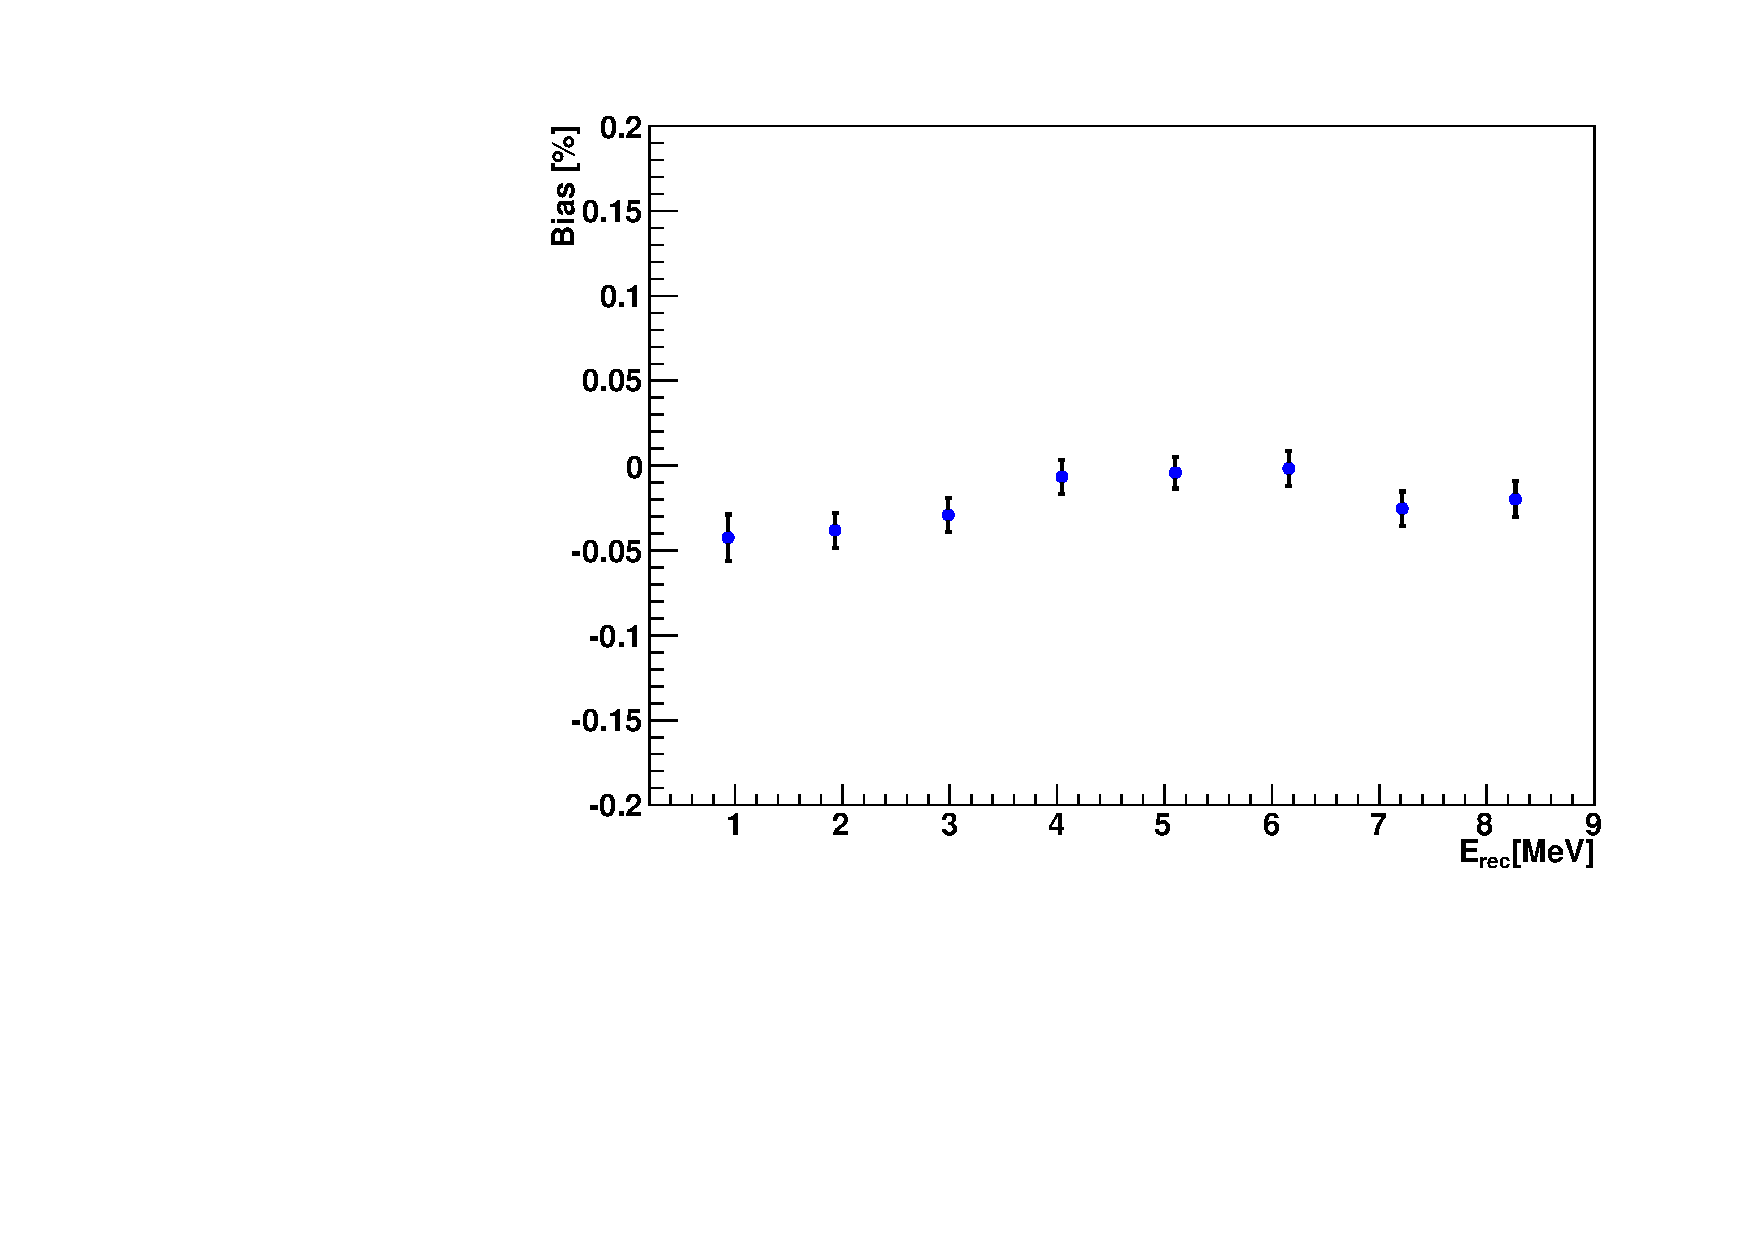
\includegraphics[width=2.5in]{non_uniform_correct_bias.pdf}
	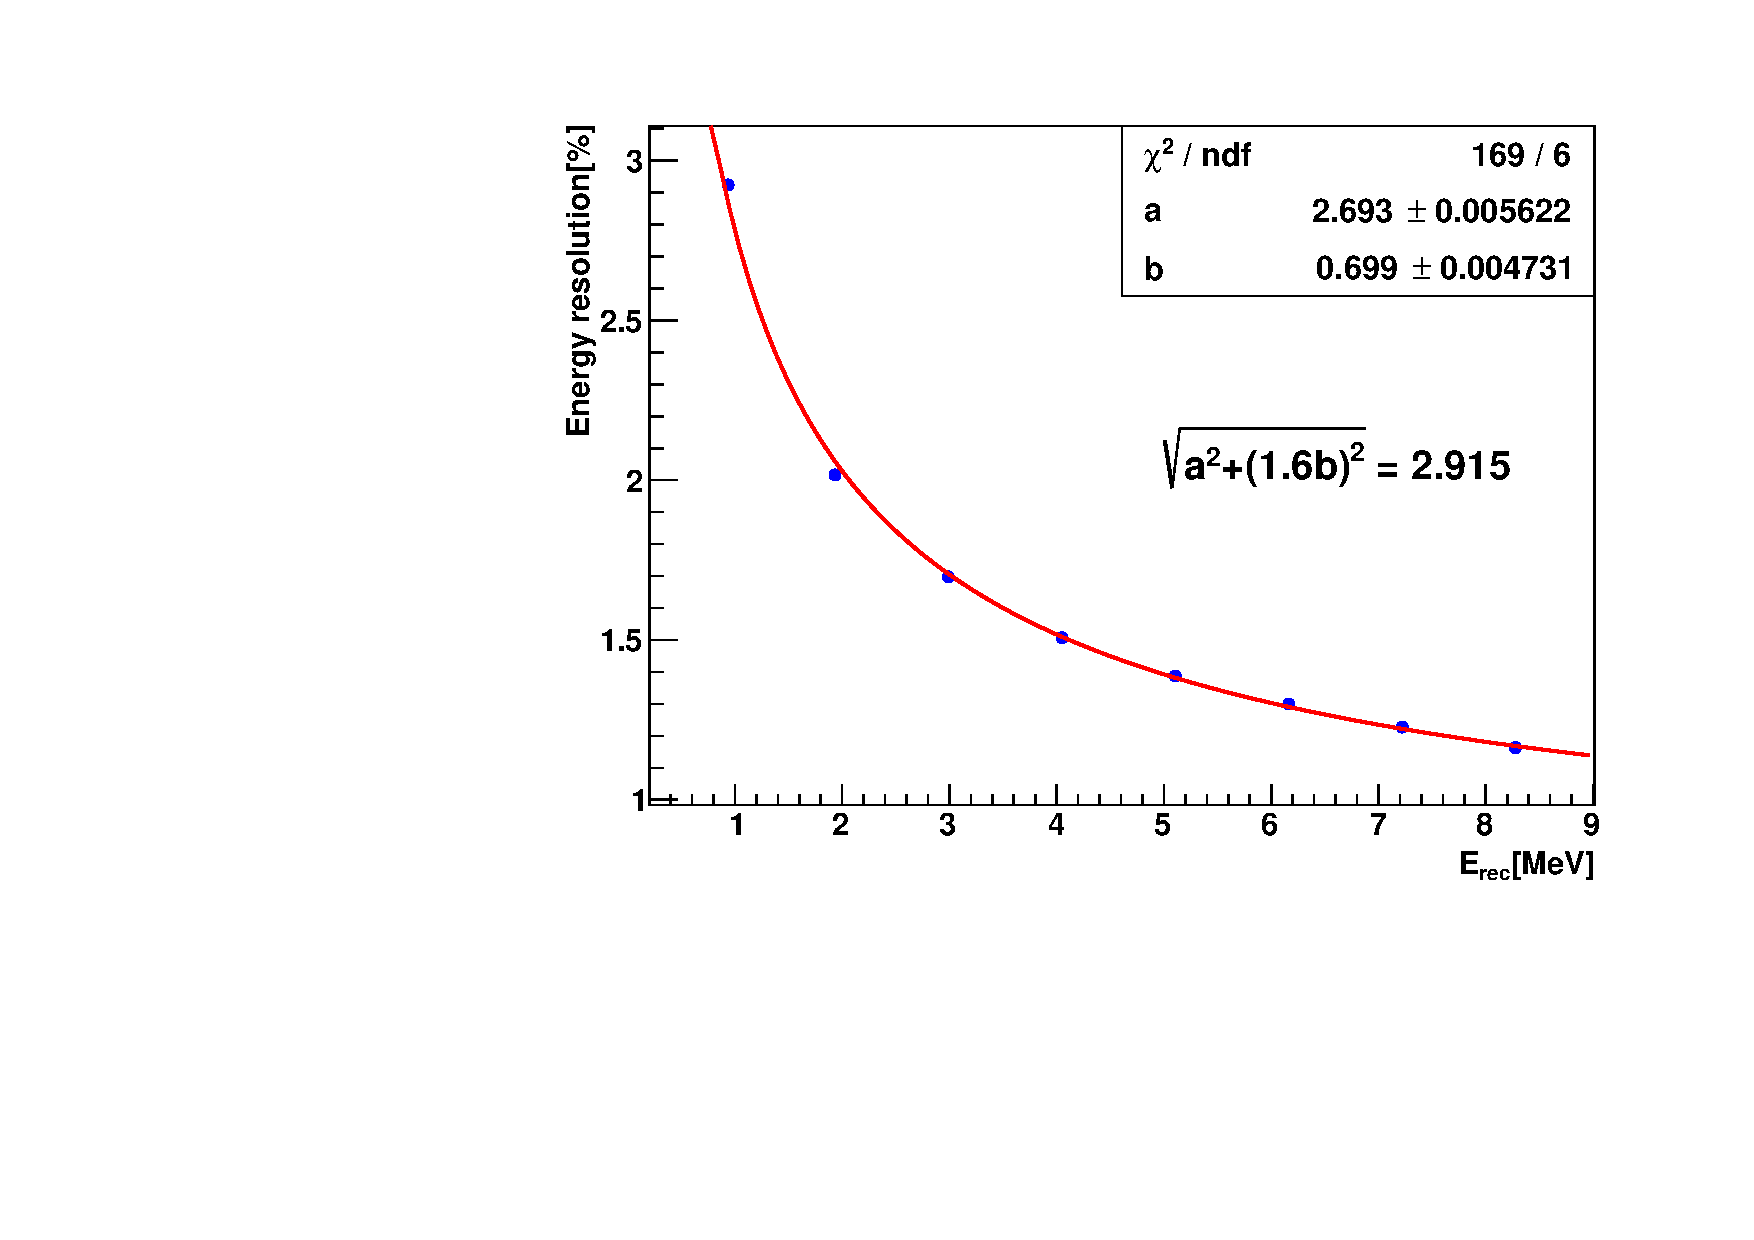
\includegraphics[width=2.5in]{non_uniform_correct_resolution.pdf}
	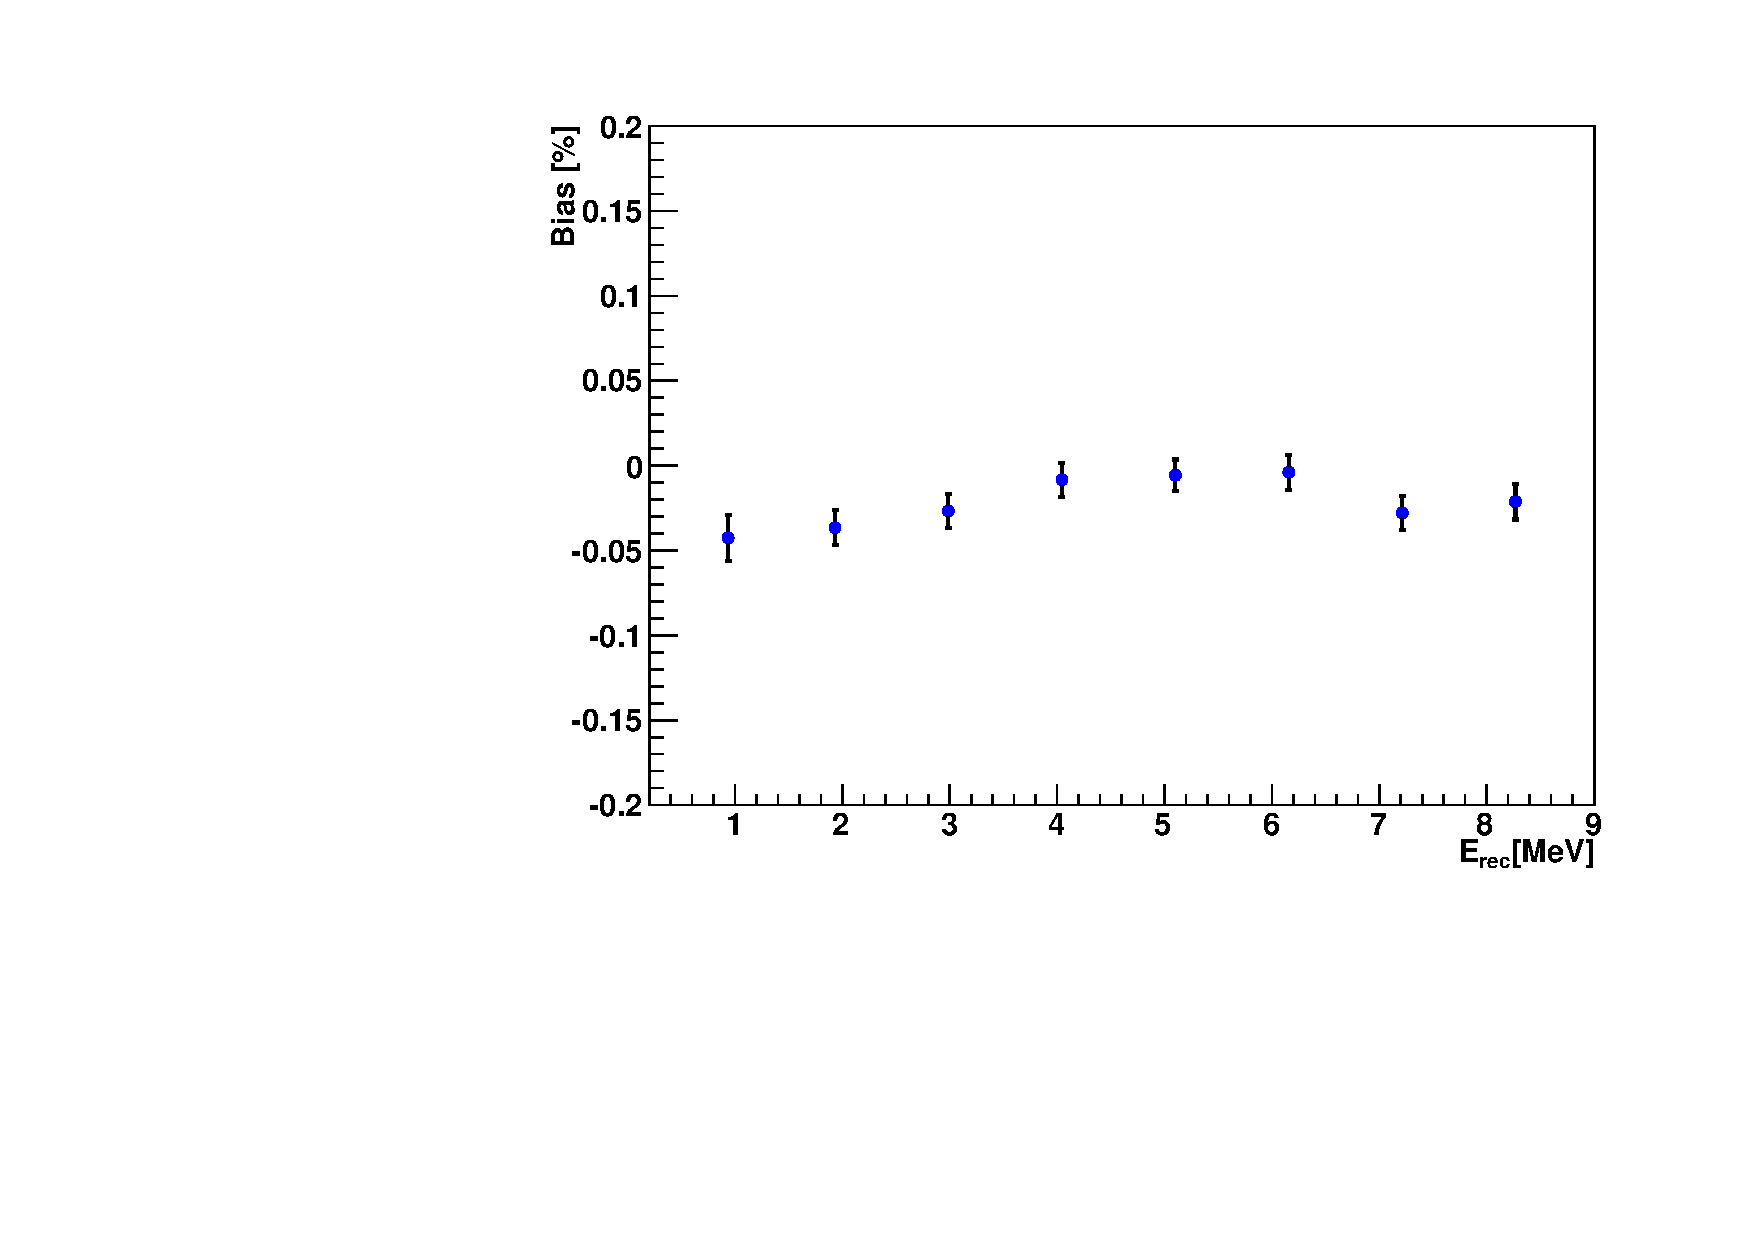
\includegraphics[width=2.5in]{bias_vertex.pdf}
	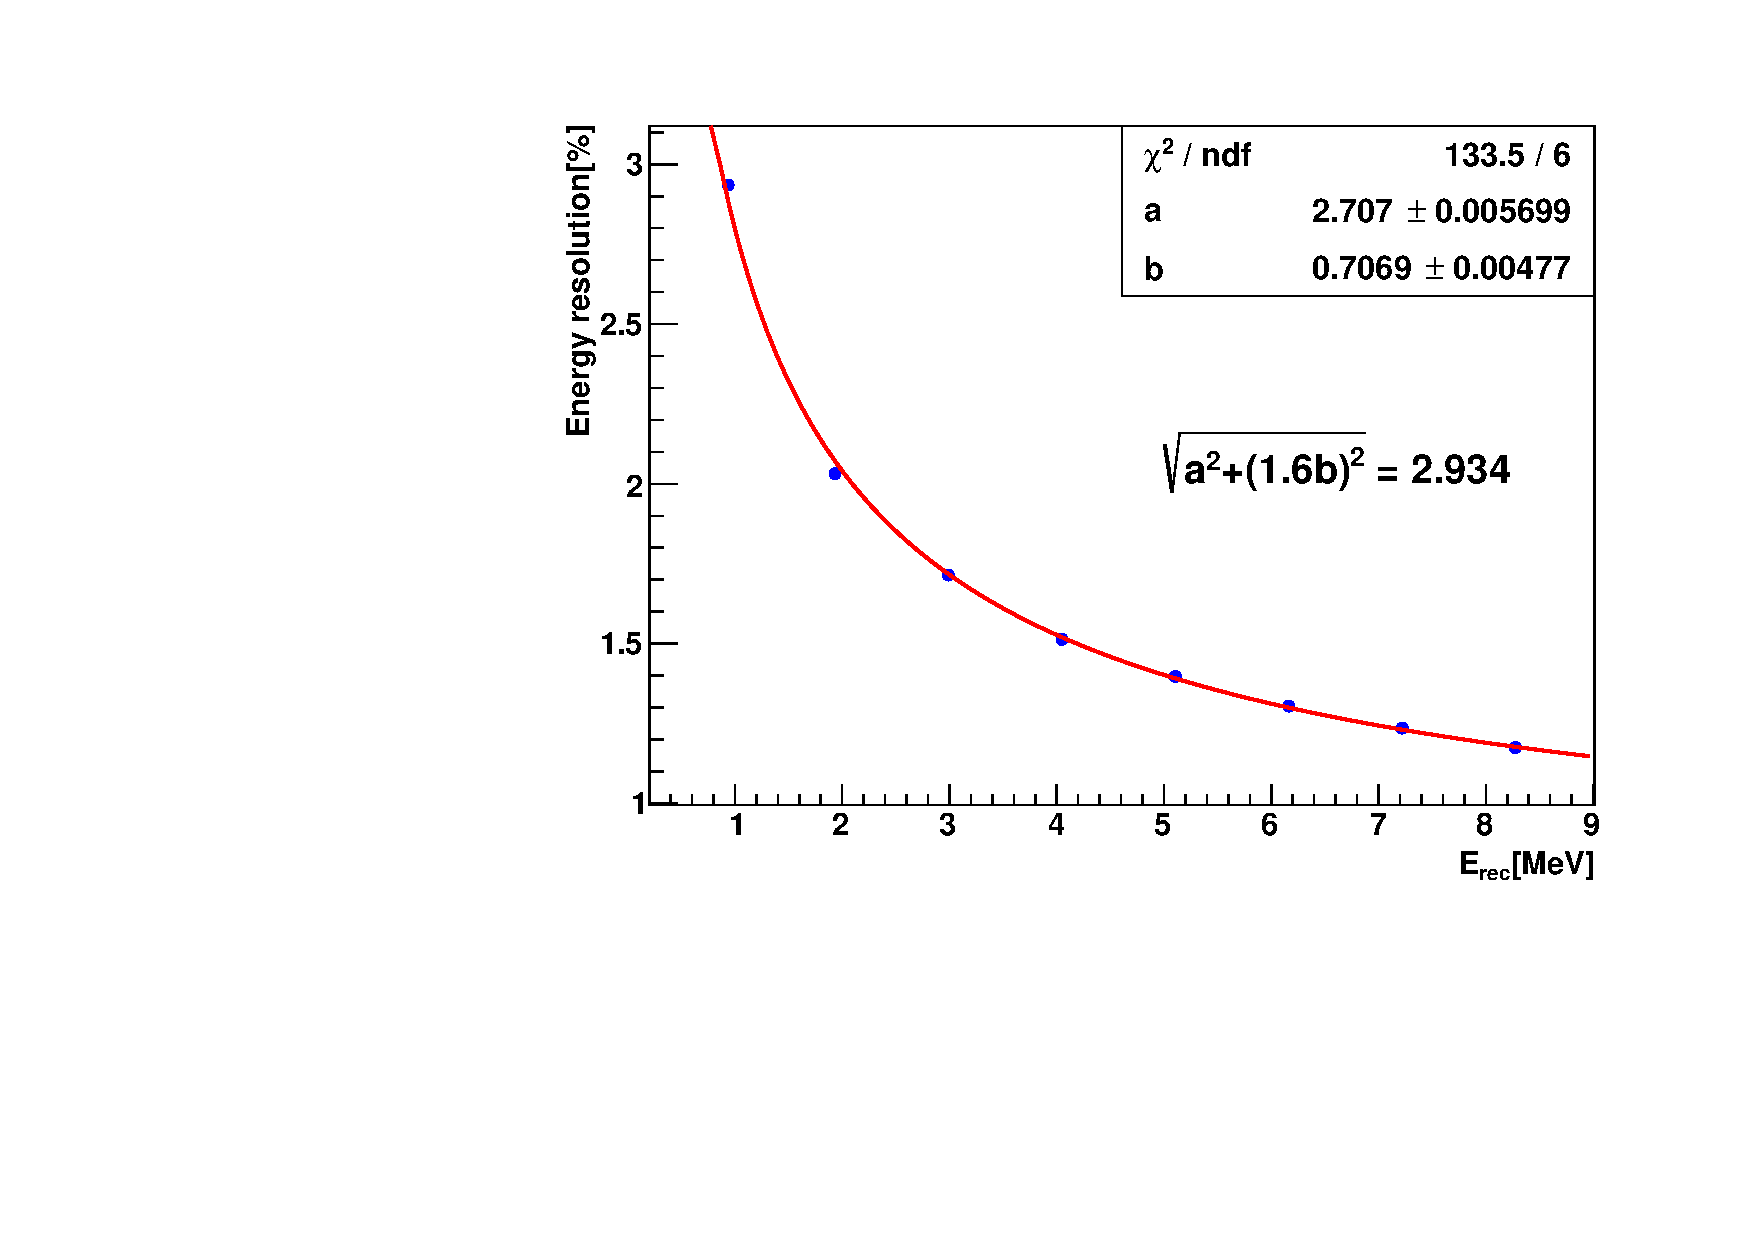
\includegraphics[width=2.5in]{resolution_vertex.pdf}
	\figcaption{non uniformity correction}
	\label{non_uniform_crrect_sum}
\end{center}

\begin{center}
	\centering
	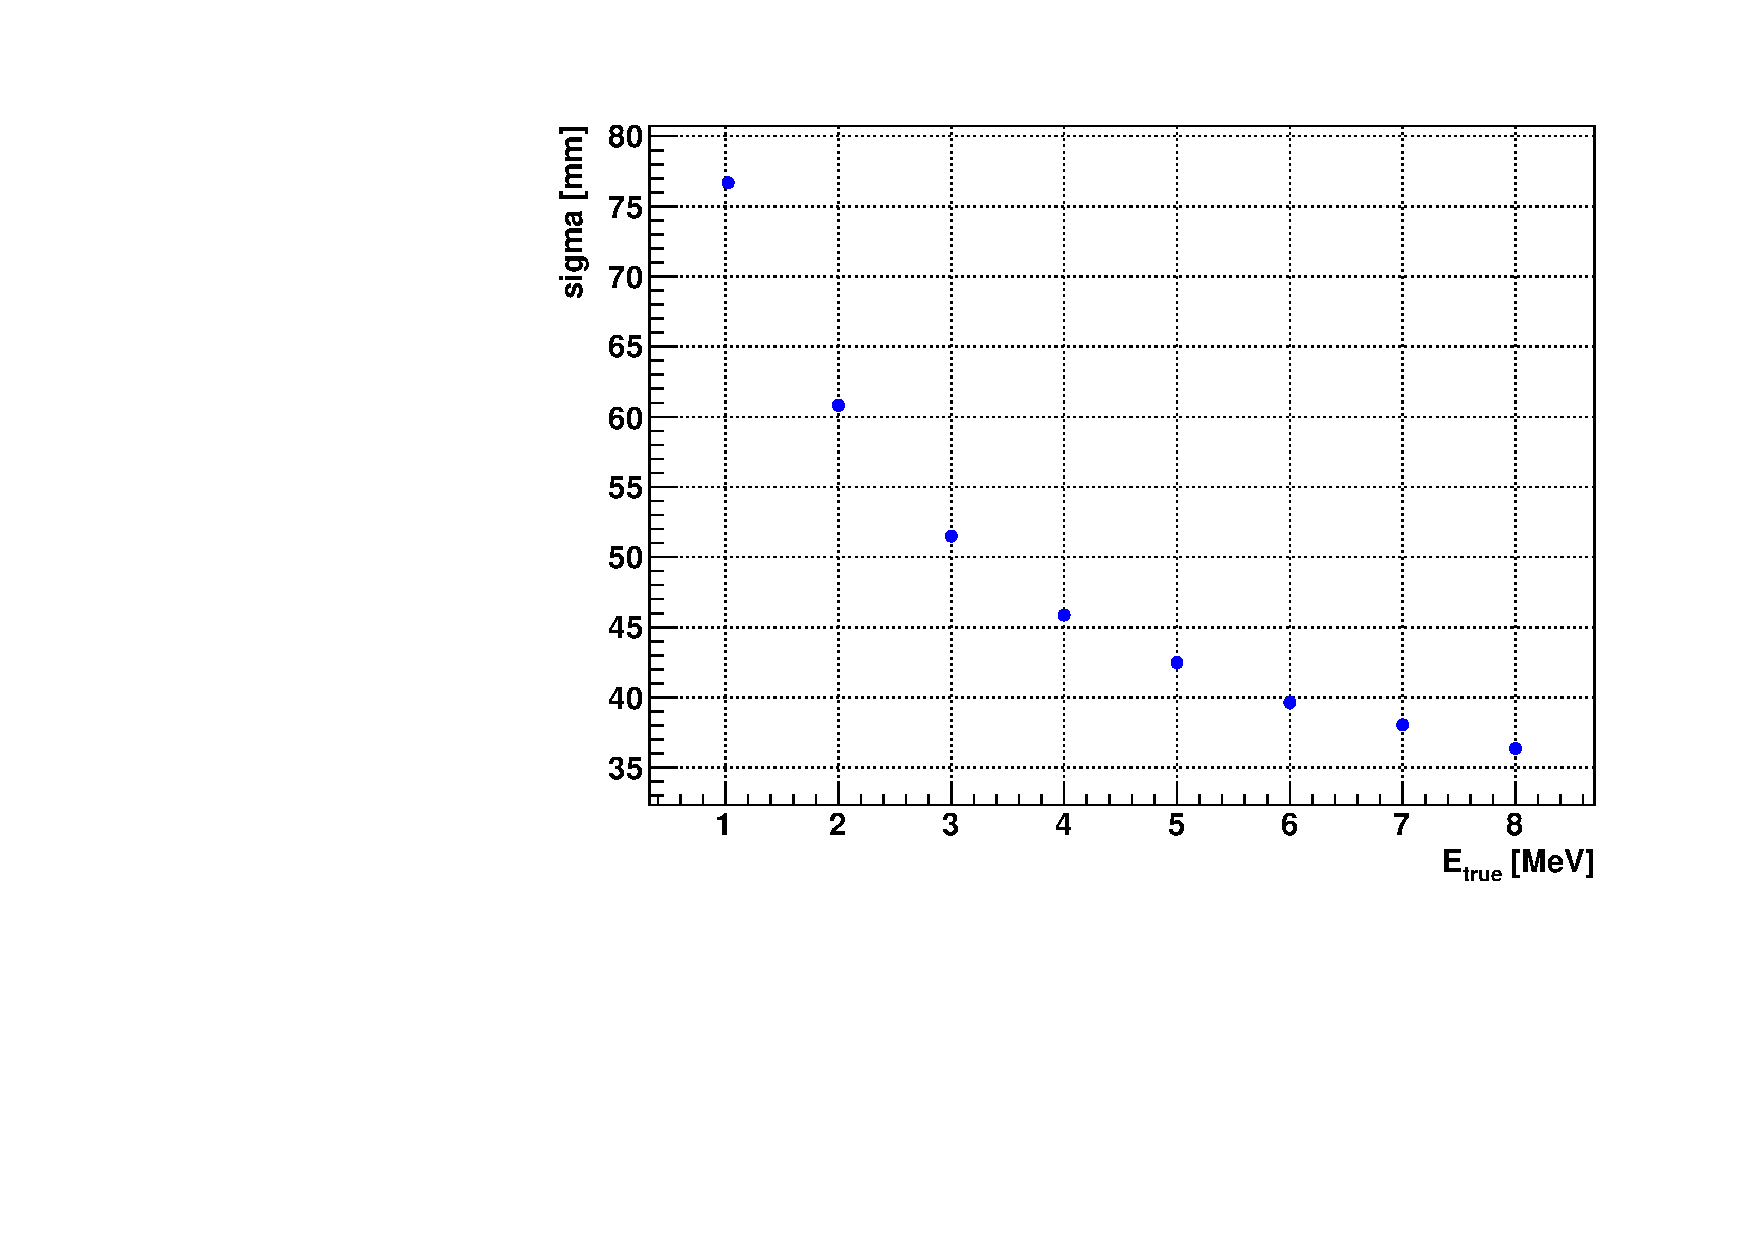
\includegraphics[width=3in]{vertex_resolution.pdf}
	\figcaption{vertex reconstruction resolution}
	\label{vertex_resolution}
\end{center}

\subsection{Basic source coverage.}
In the realistic experiments, it's impossible to use infinite points to do calibration. We purpose to do the CLS calibration monthly, and to avoid affect the normal physics data taking, the monthly calibration time should be limited to about 1 days. So the inner calibration points are 240, including 21 with ACU and 219 with CLS. We randomly select 219 points from a mount of points, and then calculate the corresponding energy resolution. Repeat the selection multiple times and then get the distribution of energy resolution. Choose the best selection with minimum energy resolution. Fig.~\ref{basic_coverage} shows relative best choice of calibration points. Fig.~\ref{non_uniform_crrect_sum} shows the result of non-uniformity correction with true vertex of IBD events and true position of calibration source. 

\subsection{Systematic uncertainty analysis.}
Vertex reconstruction. The non-uniformity correction is based on vertex of events, so vertex reconstruction significantly affects the quality of non-uniformity correction. 
Here we use the assumption of vertex reconstruction in Yellow book as shown in Fig.~\ref{vertex_resolution}. As shown in table~\ref{summary_resolution}, with vertex smearing, the overall energy resolution is 0.02\% worse than before.


\begin{center}
	\centering
	%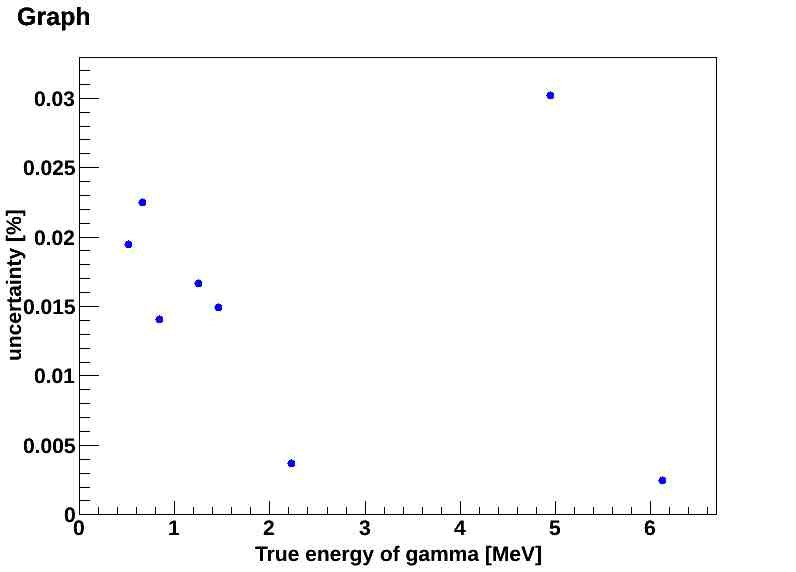
\includegraphics[width=3in]{statistical.jpg}
	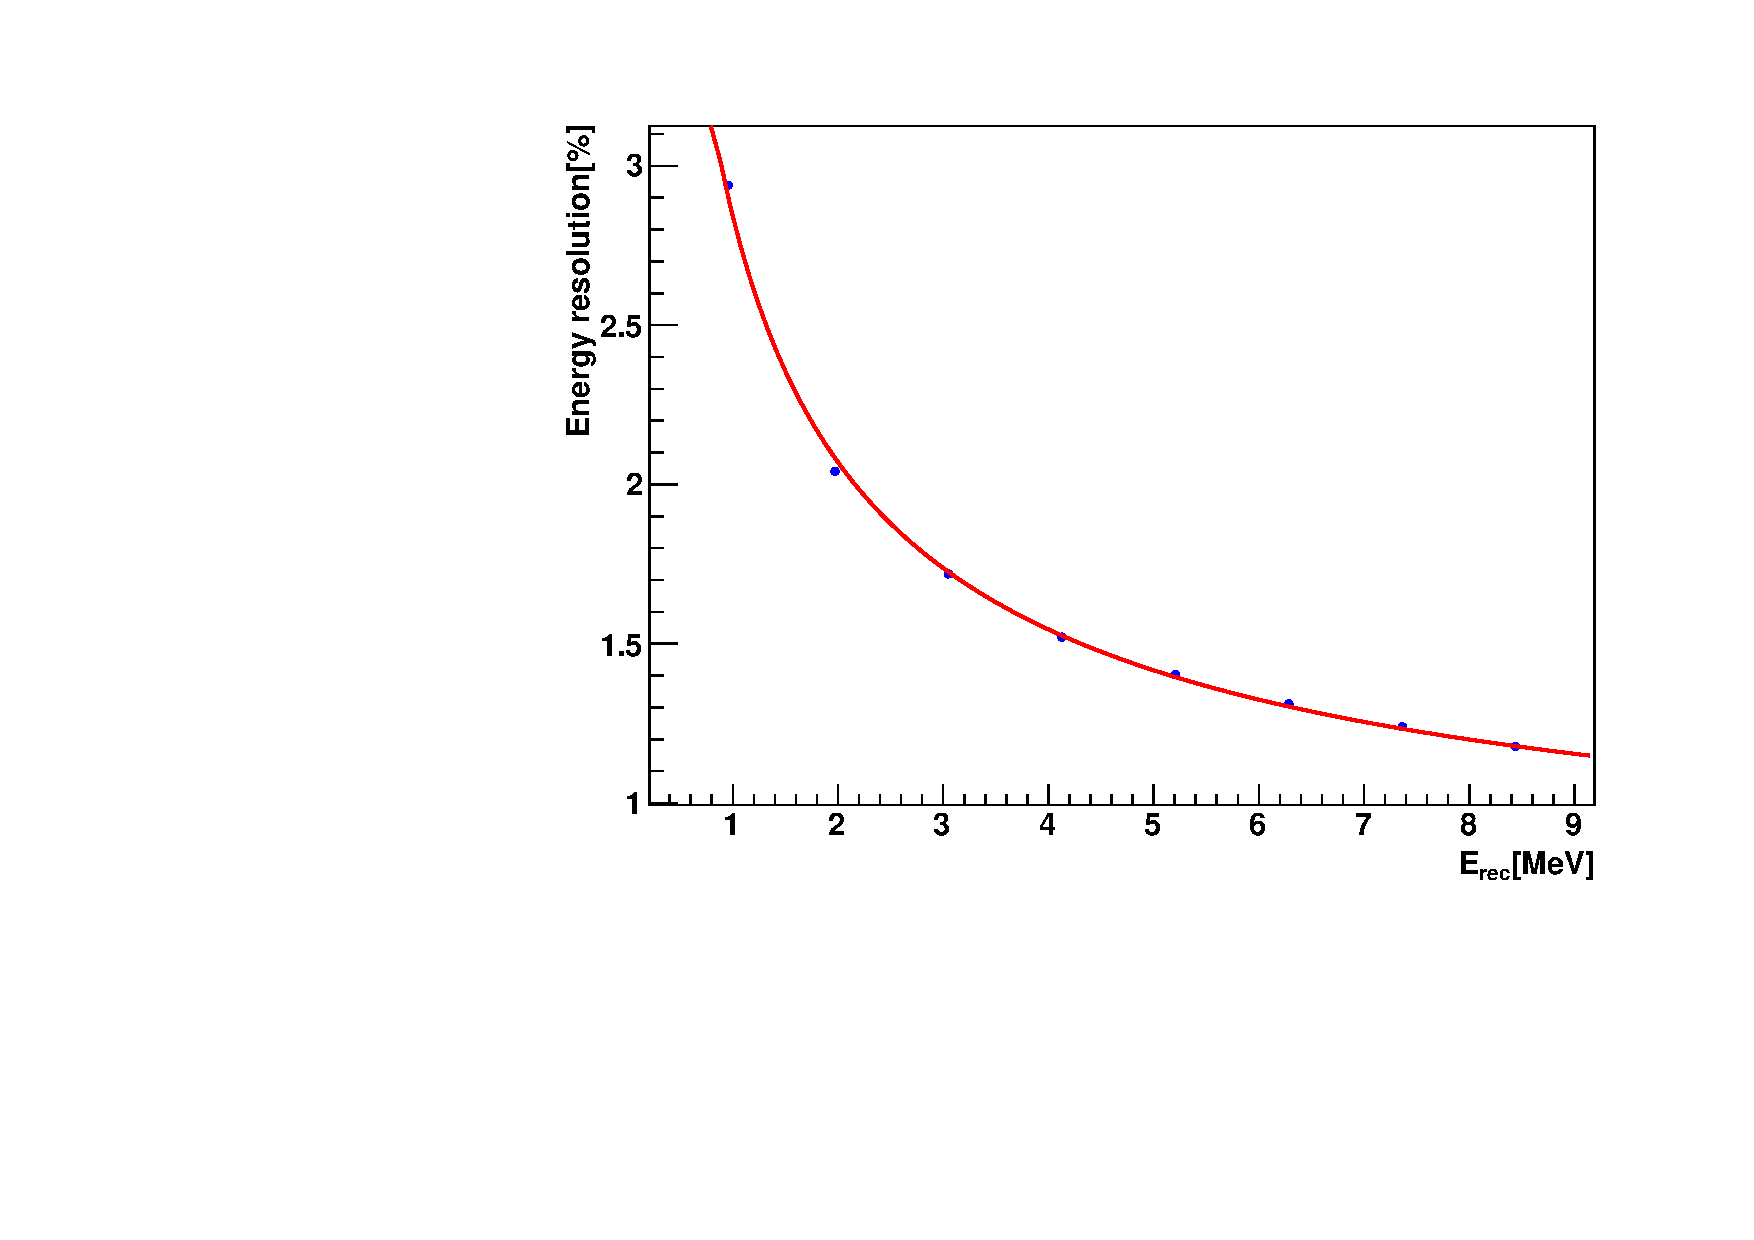
\includegraphics[width=3in]{resolution_position_smearing.pdf}
	\figcaption{a=2.75\% and b=0.70\%, and the overall energy resolution is 2.97\% }
	\label{cls_position_smearing}
\end{center}

Positioning smearing. Due to self-weight of cable and friction, it's difficult to determine position of source only based on length of cable. So an independent positioning system was purposed. In this simulation, we assume the accuracy 3 cm, which is the requirement for positioning system. To simulate this effect, we randomly smear the calibration source with 3 cm position resolution.
With position smearing for CLS calibration source, the overall energy resolution is 2.94\%, 0.01\% worse than before as shown in Fig~\ref{cls_position_smearing}.


\section{Conceptual calibration strategy}
The calibration schedule is based on above simulation result. There two types for the routine calibration, weekly calibration and monthly calibration. Also, a special calibration is necessary at the start of the experiment, which will take a relative long time.

\subsection{Weekly calibration}
The weekly calibration will be operated every week with one radioactive source and one laser, as shown in table~\ref{weekly_time}.
During the weekly calibration, only ACU will be executed.


\subsection{Monthly calibration}
The monthly calibration will be operated every month. During the monthly calibration, the ACU, CLS, and GT will be conducted. 


\end{multicols}

\begin{center}
	\tabcaption{\label{factors} Energy resolution with various factors}
	\footnotesize
	%\resizebox{\textwidth}{!}{
	\begin{tabular*}{170mm}{@{\extracolsep{\fill}}ccccccc}
		%\begin{tabular}{ccccccc}
		\toprule  % ???
		Effects & a & b& c & $\sqrt{a^{2} +(1.6b)^{2} + (\frac{c}{1.6})^{2}}$\\ 
		\hline
		%\midrule  % ???
		ideal & 2.693(5) & 0.699(5)& 0 & 2.92(1)\\
		vertex smearing &2.707(6) & 0.707(5) & 0 & 2.93(1) \\
		positioning precision & 2.716(6) & 0.711(6) & 0 & 2.94(1)\\
		dark noise & 2.716(6) & 0.711(6) & 0.9& 3.00(1)\\
		\bottomrule  % ???
		\label{summary_resolution}
	\end{tabular*}
\end{center}

\begin{center}
	\tabcaption{Time of weekly calibration}
	\footnotesize
	\begin{tabular*}{170mm}{@{\extracolsep{\fill}}ccccccc}
		\toprule  % ???
		Source&Energy [MeV]& PE& Points & Travel time [min] & Date taking time [min]&total time [min]\\ 
		\midrule  % ???
		Neutron (Am-C) & 2.22 & 2990 & 21 & 133 & 105 & 238\\
		Laser & / & 1000 - 8000 & 6 & 67 & 36 & 103 \\
		Total &/&/&/&200&141&341\\
		\bottomrule  % ???
	\end{tabular*}
	\label{weekly_time}
\end{center}



\begin{center}
	\footnotesize
	\tabcaption{Time of monthly calibration}
	\resizebox{\textwidth}{!}{
		\begin{tabular*}{170mm}{@{\extracolsep{\fill}}cccccccc}
			\toprule  % ???
			System&Source&Energy [MeV]& PE& Points & Travel time [min] & Date taking time [min]&total time [min]\\ 
			\midrule  % ???
			ACU&Neutron (Am-C) & 2.22 & 2990 & 21 & 133 & 105 & 238\\
			CLS&Neutron (Am-C) & 2.22 & 2990 & 219 & 340 & 1095 & 1435\\
			GT&Neutron (Am-C) & 2.22 & 2990 & 11 & 40 & 55 & 95\\
			Total&/&/&/&/&/&/&1768\\
			\bottomrule  % ???
	\end{tabular*}}
	\label{monthly_time}
\end{center}


\begin{multicols}{2}

\subsection{Special calibration}
	
The special calibration can be conducted at the beginning of physics data taking.
It will be relative much time to for the calibration to have a better understanding of CD including energy non-linearity and non-uniformity, as shown in table~\ref{special_time}.  
	
\section{Conclusion}

Based on the calibration system developed with ACU, CLS and GT, the simulation shows that the strategy can satisfy the physics requirement of neutrino MH determination.




\end{multicols}

\vspace{10mm}


\begin{multicols}{2}

\subsection*{Appendices A}
\begin{small}


\end{small}

\end{multicols}


\vspace{-1mm}
\centerline{\rule{80mm}{0.1pt}}
\vspace{2mm}




\begin{multicols}{2}

\begin{thebibliography}{90}

\vspace{3mm}

\bibitem{lab1}Fengpeng An et al. 2016 . Phys. G: Nucl. Part. Phys. 43 030401

%\bibitem{lab2} Tinkham M. Group Theory and Quantum Mechanics. New
%York: McGraw-Hill, 1964. 10---50

%\bibitem{lab3} Tel T. Experimental Study and Characterization of
%Chaos. Ed. Hao B. Chaos, Singapore, World Scientific, 1990. 149

\end{thebibliography}
\end{multicols}


\clearpage

\end{CJK*}
\end{document}
